\chapter{Black Holes}
\label{ch:blackholes}

Black holes are an incredible consequence of general relativity naturally arising from the study of dense distributions of matter. We find that when the mass density of a gravitational object reaches a critical limit,\footnote{To understand the requirement of high density: in Section \ref{sec:solvingeinsteinsequations}, we wrote down the \sch solution, describing a spherical symmetric distribution of matter. For the \sch spacetime, the event horizon is located for $r = 2M$, but for almost all matter distributions, this point in spacetime is within the distribution of matter where the \sch solution is no longer valid. Hence, we can only expect black holes to appear once the matter distribution is suitably dense such that all the matter is contained in a ball with radius $r < 2M$.} a region of spacetime appears in which it is impossible for causal information to escape. These regions are what we call as black holes, and their boundaries are known as event horizons. 

One of the most extraordinary advances in modern theoretical physics was the development of black hole thermodynamics. The story begins geometrically, in the development of the laws of black hole mechanics \cite{Bardeen:1973gs, Hawking:1971vc}, a set of four laws which had a remarkable similarity to the laws of thermodynamics. The relations were similar enough to lead Bekenstein to conjecture a proportionality between a black hole's area and its entropy \cite{Bekenstein:1973ur}. Through studying gravitational solutions semi-classically, Hawking was able set the constant of proportionality. Considering a curved spacetime quantum field, Hawking found that a black hole emitted thermal radiation as a black body \cite{Hawking:1974sw}, making concrete our understanding of the geometric rules derived from black holes as thermodynamic relations. The core of this thesis is work put towards better understanding this relationship between general relativity and thermodynamics. 

In this chapter, we introduce the reader to many of the tools we will need while studying the planar symmetric solutions of $\N = 2$ supergravity. We begin in Section \ref{sec:horizons}, looking at the mathematical structure of a horizon. We follow this in Section \ref{sec:gencausalstructure} by considering the causal structure of a black hole and then develop a global description of the \sch black hole. In Section \ref{sec:rnsol}, we look at the Einstein-Maxwell theory, and derive a black hole solution which is charged under the Maxwell field, known as the Reissner-Nordstr\"om solution. This is followed by a discussion of what we mean by the conserved energy of a gravitational solution in Section \ref{sec:gravitationalmass}. We follow this with an overview of the laws of black hole mechanics and their relationship to the laws of thermodynamics in Section \ref{sec:bhthermo}. In Section \ref{sec:eucldeanactionformalism}, we show using the Euclidean action formalism that one can derive thermodynamic quantities from the saddle-point approximation of the gravitational partition function, and use Reissner-Nordstr\"om black hole as a worked example.


\section{Horizons}
\label{sec:horizons}

A black hole is a region of spacetime for which it is impossible for a timelike or null curve to escape. In essence, the gravitational field is so strong, that one would need to travel faster than the speed of light to escape the region. We call the boundary of this region an \emph{event horizon}, which we understand as the point of no return. This `definition' of a black hole is sufficient to understand what we mean when we talk about a black hole, but due to the work of Hawking, Penrose and others, this definition can be made more formal. The language and tools needed to do this go beyond the scope of our discussion, and so we reference \cite{Hawking:1973uf, Wald:106274} as two key textbooks for this result. As a black hole region is impossible to escape, we realise that to properly define the event horizon, we must understand the black hole geometry globally. It is not enough to say you cannot currently escape, you have to know that whatever happens, you never will.

In this section we introduce two horizons closely related to event horizons, the Killing horizon and the trapping horizon.\footnote{The trapping horizon is the boundary of the trapping region, which we will define in better detail in Section \ref{sec:trapping}. Penrose proved the singularity theorem \cite{Penrose:1964wq}, which states that within a trapping region at least one geodesic is future-inextendible, signifying the presence of a singularity. An extraordinary result showing the physical significance of spacetime singularities.} Killing horizons are surprisingly simple to locate given a manifold's line element, and when the spacetime is stationary, Hawking showed that the event horizon is a Killing horizon \cite{Hawking:1973uf}. The trapping horizon, unlike the event horizon, can be defined locally, and we will find the notion of a trapping horizon useful when studying black hole thermodynamics. It has been proven that the trapping horizon is always contained within the event horizon \cite{Wald:106274}.


\subsection{Null hypersurfaces}

For a manifold $M$, with a metric $g$, the vector field $n^\mu = \nabla^\mu f$ is normal\footnote{Although technically the normal vector field need not be a gradient in general, see for example \cite{LopesCardoso:2019mlj}.} to a surface $\Sigma$ defined by constant $f$, for any function $f$ such that $df \neq 0$ on $\Sigma$. 

\begin{defn}
	A \emph{null hypersurface} $\N$ is a hypersurface whose normal is everywhere null.
\end{defn}

For any null hypersurface $\N$, with a normal $n_\mu$, a vector $X^\mu$ tangent to $\N$ satisfies $X \cdot n = 0$. As the normal vector is null: $n \cdot n = 0$, we see that the normal is itself a tangent vector for some null curve in $\N$.

\begin{prop}
The integral curves of the normal vector field of a null hypersurface are geodesics.	
\end{prop}
\begin{proof}
	Let $\N$ be a null hypersurface for $f = $ constant. We can write the unit normal vector $n = \tilde{f} df$, for some function $\tilde{f}$. For some general normal vector field $N = df$, $n^\mu$ and $N^\mu$ have the same integral curves. 
	
	Taking the covariant derivative of the norm of $N$ evaluated on $\N$, we can write down
	\begin{equation}
	\label{eq:geoproof1}
		\nabla_\mu (N^\nu N_\nu) |_\N = 2 N^\nu \nabla_\mu N_\nu  = 2 N^\nu \nabla_\nu N_\mu,
	\end{equation}
	where we have used that $\nabla_\nu N_\mu = \nabla_\nu \nabla_\mu f = \nabla_\mu \nabla_\nu f = \nabla_\mu N_\nu$.
	As we also know that $N^\nu N_\nu = 0$, $N^2$ is constant on $\N$. From this, we know that the gradient of $N_\mu$ is normal to $\N$
	\begin{equation}
	\label{eq:geoproof2}
		\nabla_\mu (N^\nu N_\nu) |_\N = 2 h N^\nu,
	\end{equation}
	for some function $h$. 
	Combining \eq{geoproof1} with \eq{geoproof2} we can write
	\begin{equation*}
		N^\nu \nabla_\nu N_\mu = 2 h N^\nu,
	\end{equation*}
	which we read as the geodesic equation for a non-affinely parameterised geodesic \eq{geod}. We thus see integral curves of $N^\mu$, and therefore $n^\mu$, are geodesics. Appropriately picking the normalisation of the curve parameter, one can find an affinely parameterised geodesic.
\end{proof}

\begin{defn}
The \emph{generators} of a null hypersurface $\N$ are the null geodesics $x^\mu(\lambda)$, with affine parameter $\lambda$, such that the tangent vectors to $x^\mu(\lambda)$ are normal $\N$. 
\end{defn}

\begin{defn}
	A null hypersurface $\N$ is a \emph{Killing horizon} when there exists a Killing vector $\xi^\mu$ normal to $\N$.  
\end{defn}

Hawking proved the rigidity theorem \cite{Hawking:1973uf}, which states that for a stationary black hole, the event horizon is also a Killing horizon, for a review, see \cite{Ionescu:2015dna}. We will comment again on event horizons in Section \ref{sec:gencausalstructure}, but note here that often we work with the existence of a Killing horizon rather than an event horizon, due to the simplicity in locating a Killing horizon by considering the line element of a gravitational solution.

\subsection{Surface gravity}

As $\xi^2 = 0$ on a Killing horizon, then the gradient of $\xi^2$ will also be zero along the null hypersurface. From this, we can write down the relationship \cite{Poisson:2009pwt}
\begin{equation}
\label{eq:surfacegravity}
	\nabla_\mu (\xi^\nu \xi_\nu) = -2 \kappa \xi_\mu.
\end{equation}
The function $\kappa$ is known as the \emph{surface gravity} of the Killing horizon.

Rearranging the above definition for the surface gravity by using Killing's equation, we obtain
\begin{equation*}
\begin{aligned}
		\nabla_\mu (\xi^\nu \xi_\nu) &= 2 \xi^\nu \nabla_\mu \xi_\nu, \qquad \nabla_\mu \xi_\nu + \nabla_\nu \xi_\mu = 0 \quad (\text{Killing's Equation}) \\
		&= -2 \xi^\nu \nabla_\nu \xi_\mu \\
		\xi^\nu \nabla_\nu \xi_\mu &= \kappa \xi^\mu.
\end{aligned}	
\end{equation*}
This allows us to geometrically interpret the surface gravity $\kappa$ as the measure of the failure of $\lambda$ to be an affine parameter, where $\xi^\mu = \partial_\lambda$. We see that the Killing vector $\xi^\mu$ obeys the non-affine geodesic equation \eq{geod}.

We can understand the surface gravity from another perspective. Let us imagine a spaceship at rest in some static, asymptotically flat spacetime, some distance above the Killing horizon. To maintain its position within space, we can intuitively understand the spaceship as accelerating so as not to fall towards the black hole. To use a more formal language, a particle at rest in a static spacetime follows the orbit of a timelike Killing vector field $k^\mu$. As these orbits are not geodesics, we understand this particle as accelerating. 

Now instead of imagining the ship's acceleration being generated by its engines, let us imagine the ship is held in place by some rigid rod extending off to an anchor point at infinity. An observer at infinity measures the force holding the ship in place as a tension $T$ in the rod. In the limit of the spaceship being located on the Killing horizon, the tension measured at the anchor point tends towards the surface gravity: $T \to \kappa$. We can then say that the surface gravity $\kappa$ is the force needed to hold a body in place on the Killing horizon for an observer at infinite distance. The local force experienced by the spaceship is a different matter. The local tension, \ie the force exerted by the ship onto the rod, diverges as the ship approaches the Killing horizon. Note for this interpretation, we have required the spacetime to be static. For rotating solutions, such as the Kerr solution \cite{Kerr:1963ud}, this interpretation is no longer valid.


\subsection{Expansion of null hypersurfaces}
\label{sec:expansionnullhyper}
In Section \ref{sec:congruences}, we discussed geodesic congruences and showed the gauge freedom for the affine parameter was fixed for timelike and spacelike congruences by setting $U \cdot S = 0$. For null congruences, we need to fix the gauge freedom by constraining the action of $S$ on two vector fields. In the following discussion, we look at a congruence containing the generators of a null hypersurface $\N$. In this case, the displacement vector is tangent to $\N$ such that $U \cdot S$ = 0 always holds.

To see how to set the gauge freedom, let us choose a spacelike hypersurface $\Sigma$ which intersects each geodesic of the congruence only once. We define our second vector field $N^\mu$ such that on the hypersurface we have
\begin{equation*}
	N^2 = 0, \qquad N \cdot U = -1.
\end{equation*}
We can understand $N^\mu$ as a vector field in $M$ by extending it off $\Sigma$ through parallel transport along $U^\mu$: $\nabla_U N^\mu = 0$. If $U^\mu$ is tangent to outgoing radial null geodesics, we understand $N^\mu$ as tangent to ingoing radial null geodesics, and vice-versa.

Given our two vector fields $N$ and $U$, we can now fix the gauge freedom in $\lambda$ by picking the displacement vector such that
\begin{equation*}
	U \cdot S = 0, \qquad N \cdot S = 0.
\end{equation*}
Under this condition, the displacement vector $S^\mu$ spans a two-dimensional subspace tangent to both $U^\mu$ and $N^\mu$. We can define a projection onto this tangent space using
\begin{equation*}
\tensor{P}{^\mu_\nu} = \tensor{\delta}{^\mu_\nu} + N^\mu U_\nu + U^\mu N_\nu,
\end{equation*}
and we will refer to the projected quantities using a hat
\begin{equation*}
	\tensor{\hat{B}}{^\mu_\nu} = \tensor{P}{^\mu_\rho} \tensor{B}{^\rho_\sigma} \tensor{P}{^\sigma_\nu}.
\end{equation*}
We note that for null congruences which do not contain generators of a null hypersurface \ie when the displacement vector is not tangent to the hypersurface, we would have to project the displacement vector, 
\begin{equation*}
	\hat{S}^\mu = \tensor{P}{^\mu_\nu} S^\nu, \qquad S^\mu = \alpha U^\mu + \beta N^\mu + \hat{S}^\mu,
\end{equation*}
where we have additionally written out the form of the displacement vector for a generic null congruence.

We can interpret $\tensor{\hat{B}}{^\mu_\nu}$ as a matrix in the two-dimensional space tangent to $U^\mu$ and $N^\mu$. We can decompose this matrix into its algebraically irreducible pieces
\begin{equation*}
	\tensor{\hat{B}}{^\mu_\nu} = \half \theta \tensor{P}{^\mu_\nu} + \tensor{\hat{\sigma}}{^\mu_\nu} + \tensor{\hat{\omega}}{^\mu_\nu},
\end{equation*}
where we have split the matrix into its trace, traceless symmetric and anti-symmetric parts: 
\begin{equation*}
\begin{aligned}
	\theta &= \tensor{\hat{B}}{^\mu_\mu}, & &\qquad \textit{Expansion}, \\
	\tensor{\hat{\sigma}}{_{\mu\nu}} &= \tensor{\hat{B}}{_{(\mu\nu)}} - \half P_{\mu \nu} \tensor{\hat{B}}{^\rho_\rho} & &\qquad \textit{Shear}, \\
	\tensor{\hat{\omega}}{_{\mu \nu}} &= \tensor{\hat{B}}{_{[\mu\nu]}} & &\qquad \textit{Twist}.
\end{aligned}
\end{equation*}
We interpret these values in the following way. Let us take two vector fields $V_\pm^\mu$ which are orthogonal to $U^\mu$ and $N^\mu$. The two vectors $V_\pm^\mu$ define an area element in the space tangent to both $U^\mu$ and $N^\mu$ given by the expression
\begin{equation*}
		A = \varepsilon^{\mu \nu \rho \sigma} U_\mu N_\nu V_{+ |\rho} V_{- |\sigma}.
\end{equation*}
The \emph{shear} measures the change of shape of this area while maintaining its magnitude. We can think of this as describing the geodesics moving apart in one direction and towards each other in another. The \emph{expansion}, measures the change in the magnitude of the area. When $\theta > 0$, we say understand that the geodesics are moving away from each other (expanding) and for $\theta  < 0$ they come together (contraction). To see how the expansion measures the change in the area,, we can vary the area $A$ with respect to our affine parameter to find:
\begin{equation*}
\begin{aligned}
\diff{A}{\lambda} &= U \cdot \nabla A = \varepsilon^{\mu \nu \rho \sigma} U_\mu N_\nu \left[U \cdot \nabla \left(V_{+ |\rho} V_{- |\sigma} \right) \right], \\
&= \varepsilon^{\mu \nu \rho \sigma} U_\mu N_\nu \left[ \tensor{\hat{B}}{^\lambda_\rho} V_{\lambda | +} V_{\sigma | -} + \tensor{\hat{B}}{^\lambda_\sigma} V_{\lambda | +} V_{\rho | -}  \right] ,\\ 
&= \varepsilon^{\mu \nu \rho \sigma} U_\mu N_\nu \tensor{\hat{B}}{^\lambda_\rho} \left( V_{\lambda | +} V_{\sigma | -} - V_{\sigma | +} V_{\lambda | -} \right), \\ 
&= \varepsilon^{\mu \nu \rho \sigma} U_\mu N_\nu \tensor{\hat{B}}{^\lambda_\lambda} V_{\rho | +} V_{\sigma | -} = A \theta.
\end{aligned}
\end{equation*}
From this, we can then understand the expansion as measuring the rate of increase of the area with respect to the affine parameter $\lambda$.

The \emph{twist} $\hat{\omega}_{\mu \nu}$, measures how the geodesics twist around each other. For congruences containing the generators null hypersurface $\N$, the twist is everywhere zero on $\N$. If $\hat{\omega}_{\mu \nu} = 0$, then $U^\mu$ is hypersurface orthogonal \cite{Wald:106274}. 

An alternative and useful expression for the expansion is given by
\begin{equation}
\label{eq:genexpansion}
	\theta = \nabla_\mu U^\mu = g^{\mu \nu} \nabla_\mu U_\nu,
\end{equation}
which can be derived from
\begin{equation*}
	\theta = \tensor{P}{^\mu_\nu} \tensor{B}{^\nu_\rho} \tensor{P}{^\rho_\mu},
\end{equation*}
expanding out all the terms and using that
\begin{equation*}
	 \qquad U^\mu \nabla_\mu U^\nu =  U^\mu \nabla_\nu U^\mu = 0.
\end{equation*}
This representation of the expansion shows us that $\theta$ is independent of the vector field $N^\mu$ and should be understood as an intrinsic property of the congruence. 

Later when discussing the laws of black hole mechanics, we will consider a congruence containing the generators of a Killing horizon. With this additional property for the vector fields, we find that on the Killing horizon, all of these quantities vanish.

\begin{prop}
The expansion, shear and rotation for a geodesic congruence containing the generators of a Killing horizon are all zero evaluated on the Killing horizon: $\theta = \hat{\sigma} = \hat{\omega} = 0$.
\end{prop}

\begin{proof}
	As the generators of the Killing horizon are hypersurface orthogonal, the rotation $\hat{\omega} = 0$, as discussed before. What remains is to show that the symmetric part of $\hat{B}_{(\mu \nu)} = 0$. We denote the Killing vector field  $\xi^\mu$, which is normal to the Killing horizon $\N$. On $\N$, we can relate the Killing vector field to tangents of the generators of the hypersurface $U^\mu$ with some generic function $h$ on the hypersurface: $\xi^\mu = h U^\mu$. 
		
	To calculate the expansion and shear, we use that our Killing horizon is specified by the zero of some function $f = 0$. This allows us to write down the generator 
	\begin{equation*}
		U^\mu = h^{-1} \xi^\mu + f V^\mu,
	\end{equation*}
	for some vector field $V^\mu$. Taking the covariant derivative, we find
	\begin{equation*}
		B_{\mu \nu} = \nabla_\mu U_\nu = \partial_\mu(h^{-1}) \xi_\nu + h^{-1} \nabla_\mu \xi_\nu + \partial_\mu(f) V_\nu + f \nabla_\mu V_\nu,
	\end{equation*}
	Taking only the symmetric part, and evaluating on the hypersurface, we find
	\begin{equation*}
		B_{(\mu \nu)} \big|_{\N} = \xi_{(\nu} \partial_{\mu)} h^{-1} +  V_{(\nu} \partial_{\mu)} f,
	\end{equation*}
	where we have used Killing's Equation \eq{killings} and that $f = 0$. However, when we project this onto the orthogonal space $T_\perp$ we see that all terms vanish
	\begin{equation*}
		\hat{B}_{(\mu \nu)} = \tensor{P}{^\rho_\mu} B_{(\rho \sigma)} \tensor{P}{_\nu^\sigma} = 0,
	\end{equation*}
	as both the Killing vector $\xi^\mu$ and the derivative $\partial_\mu f$ are parallel to the vector field $U^\mu$. 	
\end{proof}


\subsection{Trapping and apparent horizons}
\label{sec:trapping}
For an observer in a spacetime, how can they decide if they're within a black hole region? The event horizon is defined as a region of spacetime in which it is impossible to send a signal to infinity. The requirement of properly dealing with \emph{impossible} and \emph{infinity} necessitates a global description for the spacetime. For certain solutions, we may only have a local patch of the solution we wish to probe, and in these scenarios, we cannot describe the black hole region.

A \emph{trapping horizon} is a way to talk about the local structure of a spacetime. It is the boundary of a trapping region, which can be thought of as a local analogue of a black hole region. Let us pick a spacelike hypersurface $\Sigma$ within our spacetime, and on that, identify a closed hypersurface $S$. For every point on $S$, we have two future-directed null vector fields $\ell^\mu_\pm$ which correspond to two families of null geodesics. We can understand each family of geodesics generating two null hypersurfaces $\N_+$ and $\N_-$. In the cases we are concerned with, null geodesics with tangents $\ell_\pm$ will correspond to the ingoing and outgoing light rays within the spacetime. We can identify a trapped surface by calculating the expansion of these vector fields.

\begin{defn}
A closed, spacelike hypersurface $S$ is a \emph{trapped surface} if both families of null geodesics orthogonal to the hypersurface have an everywhere negative expansion. When the expansions are everywhere non-positive, we say that this surface is \emph{marginally} trapped.
\end{defn}

Looking at the spacelike hypersurface $\Sigma$, we can find the \emph{trapped regions} $\mathcal{T}$ by looking at the union of all trapped surfaces $S \subset \Sigma$. The boundary of this region is called the \emph{apparent horizon} $\mathcal{A} = \partial \mathcal{T}$. Calculating the expansions on the apparent horizon, we find that it is a marginally trapped surface.

\begin{defn}
Using the foliation of a spacetime $M$ with codimension-one spacelike hypersurfaces $\Sigma_t$, one can find the set of all trapped regions $\mathcal{T}_t$. The set of their boundaries $\mathcal{A}_t = \partial \mathcal{T}$ are the codimension-two apparent horizons. We define the \emph{trapping horizon} $\mathcal{T}_{\Ham}$ as the union of all apparent horizons. 
\end{defn}

It can be shown that if weak cosmic censorship conjecture is correct, then the trapping region is contained within the black hole region \cite{Hawking:1973uf}. This implies that the apparent horizon, and hence the trapping horizon, lies either on or inside of the event horizon. Thus, we understand that if a local observer measures the existence of a trapped surface, and hence the apparent horizon, they can conclude that they lie within the black hole region.

\begin{figure}[!h]
\centering
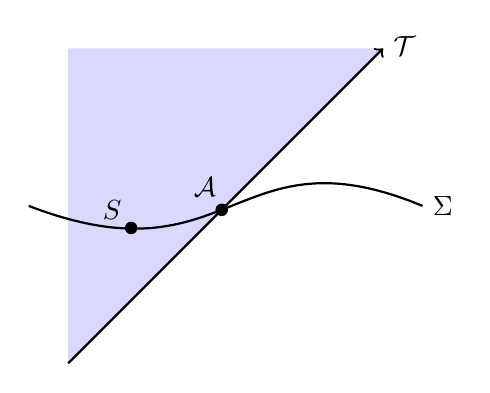
\begin{tikzpicture}
\fill[blue!15!white] (-2,-2) -- (-2,2) -- (2,2);
\draw[thick, ->] (-2,-2) -- node[at end, right]{$\mathcal{T}_{\Ham}$} (2,2);
\draw[thick] (-2.5,0) .. controls(0.1,-1) and (0.1,1) .. (2.5,0) node[at end, right] {$\Sigma$};
\node at (-0.05,-0.05) [circle,fill,inner sep=1.6pt]{};
\node at (-1.2,-0.28) [circle,fill,inner sep=1.6pt]{};

\node[above left] at (0,0){$\mathcal{A}$};
\node[above left] at (-1.2,-0.3){$S$};

\end{tikzpicture}
\label{fig:trappinghorizon}
\caption[Illustration of a trapping horizon in a spacetime $M$.]{Illustration of a trapping horizon in a spacetime $M$. $\Sigma$ is a codimension-one spacelike hypersurface. A trapped surface $S$ is a closed codimension-two spacelike hypersurface on $\Sigma$. The union of all trapped surfaces along $\Sigma$ is the trapped region $\mathcal{T}$, it's boundary is the apparent horizon $\mathcal{A}$. Evolving to the past and future from $\Sigma$ yields a set of trapped regions, shaded blue, the boundary of this region is the trapping horizon $\mathcal{T}_\Ham$.}
\end{figure}


\subsection{Classification of trapping horizons}
\label{sec:horizonclassify}
By considering the signs of the expansion of future-directed ingoing and outgoing null vector fields $\ell_\pm$, we can write down four distinct trapping horizons based on the work of \cite{Binetruy:2014ela, Helou:2015zma}. Denoting the expansions of $\ell_\pm$ as $\theta_\pm$, we distinguish the horizons in the following way. We say a trapping horizon is a \emph{future horizon} when $\theta_+ = 0$ and $\theta_- < 0$ on $\mathcal{T}_\Ham$, and a \emph{past horizon} when  $\theta_- = 0$ and $\theta_+ > 0$ on $\mathcal{T}_\Ham$. We can further distinguish trapping horizons by considering how the sign of $\theta_\pm$ changes as we cross the horizon in the direction of $\ell_\mp$. We can calculate this sign with the Lie derivative: $\La_{\ell_\mp} \theta_\pm$, evaluated on the horizon. When $\La_{\ell_\mp} \theta_\pm < 0$, we say that the horizon is an \emph{outer horizon}. Using the convention that the non-trapping region bounded by this horizon has $\theta_+ > 0$ and $\theta_- <0$, we say that the horizon is an \emph{inner horizon} when $\La_{\ell_\mp} \theta_\pm > 0$. In summary, we can identify the four types of horizons as:
\begin{enumerate}[(i)]
\item
Future outer horizons: $\theta_+ =0, \; \theta_- <0, \; \La_{\ell_-}\theta_+ <0$. The sign of $\theta_+$ changes from positive to negative with increasing $\ell_-$. We understand that `outside the horizon', the outgoing congruence is expanding, while `inside the horizon' both congruences contract. Therefore future outer horizons can be taken as local definitions of black holes. 
\item
Past outer horizons: $\theta_-=0, \; \theta_+ >0, \; \La_{\ell_+} \theta_-<0$. The sign of $\theta_-$ changes from positive to negative with increasing $\ell_+$. We understand that `outside the horizon' the ingoing congruence is expanding, while `inside the horizon' both congruences expand. We can understand outer horizons as local definitions of white holes.\footnote{We discuss white holes in some more detail in Section \ref{sec:scheddington}, but for now we can understand them as the time-reversal of a black hole.} 
\item
Future inner horizons: $\theta_+= 0, \; \theta_-<0, \; \La_{\ell_-}\theta_+ >0$. The sign of $\theta_+$ changes from negative to positive with increasing $\ell_-$. The inside region is non-trapping while in the outside region, both congruences contract. We can understand future inner horizons as the local definition of contracting cosmologies, where all null congruences become converging for large enough distances from the observer.
\item
Past inner horizons: $\theta_-=0, \; \theta_+ >0, \; \La_{\ell_+} \theta_->0$. The sign of $\theta_-$ changes from positive to negative with increasing $\ell_+$. The interior region is non-trapping while in the exterior region both congruences expand. We can therefore understand past inner horizons as a local definition of expanding cosmologies, where all null congruences become expanding for large enough distances from the observer. 
\end{enumerate}
We will return to these classifications when we discuss the temperature associated to trapping horizons.

\subsection{Vaidya spacetime}

We now take a brief detour to consider an example which illustrates a case when the event horizon and trapping horizon do not coincide, following a discussion from \cite{Poisson:2009pwt}. 

Let us consider a spherically symmetric black hole that for some finite time absorbs some null dust, increasing the mass of the black hole. Taking the \sch and allowing the mass to be a function of the null coordinate $v$, we obtain the \emph{ingoing Vaidya solution} with a line element in Eddington-Finkelstein coordinates given by \cite{Vaidya:1951zz}
\begin{equation*}
	ds^2 = -\left( 1 - \frac{2 M(v)}{r}\right) dv^2 + 2 dv dr + r^2 d\Omega^2.
\end{equation*}
This is a solution to Einstein's equations describing null dust which itself can be understood as a pressureless fluid. We assume that the black hole absorbs this null dust for a finite interval, where the mass parameter of the solution is given by
\begin{equation*}
	M(v) = 
\begin{cases} 
M_1, \qquad v \leq v_1, \\
M(v), \quad v_1 < v < v_2, \\
M_2, \qquad v \geq v_2. \\
\end{cases}	
\end{equation*}
We assume $M_2 > M_1$ and that the growth of $M(v)$ is smooth. In \cite{Poisson:2009pwt}, the expansion for the null congruences is computed and it can be shown that the apparent horizon is always located at $r = 2M(v)$. 

The event horizon for $v > v_2$ is, as expected, located at $r = 2M_2$, where we can consider this as the \sch solution of mass $M = M_2$. The surprising result comes at $v < v_2$. The event horizon is the causal boundary from future null infinity and so is located for $r = 2M_2$ throughout the spacetime, as it is the null hypersurface extending from the result of $v > v_2$. We see that the location of the event horizon requires all future knowledge of some non-stationary system, which is in direct contrast to the locations of the apparent horizons which we can compute given any time slicing.

For $v > v_2$, when there is no longer any dynamic changes to the solution, it should be clear that the trapping and event horizons coincide. However, for $v < v_2$, the horizons are distinct, with the trapping horizon contained within the event horizon. We can then understand that some observer within the spacetime could locally measure themselves as exterior to the Trapping horizon, but ultimately still unable to escape the black hole region if they are interior to the event horizon. An illustration of this is given in Figure \ref{fig:vaidya}.

\begin{figure}[!h]
\centering
\begin{tikzpicture}
\draw[thick, gray, dashed] (-2,-2) -- node[at end, right, black]{$\mathcal{H}^+_1$} (2,2);
\draw[thick] (0,-2) -- node[at end, right]{$\mathcal{H}^+_2$} (4,2);
\draw[thick, blue] (-2,-2) to[out=45, in=-135] coordinate[pos=.5] node[at start, right, black]{$\; \; \;\mathcal{T}_\Ham$}(4,2);
\node at (0.25,-1) [circle,fill,inner sep=1pt]{};

\end{tikzpicture}
\caption[An illustration of the horizons for a Vaidya black hole solution being irradiated by a null dust]{An illustration of the horizons for a Vaidya black hole solution being irradiated by a null dust. The dashed event horizon $\Ham_1^+$ would be the boundary if the mass remained at $M = M_1$. The blue curve depicts the trapping horizon built from the union of apparent horizons each located for $r = 2M(v)$. The event horizon $\Ham_2^+$ is the boundary of the causal past of future null infinity and is determined by the final mass $M_2$ of the solution. We see that an observer $\Op$ (depicted as a point) outside of the trapping horizon in this non-stationary solution can still be trapped within the black hole.}
\label{fig:vaidya}
\end{figure}

\section{Causal structure of black holes}
\label{sec:gencausalstructure}
In this section, we use the Schwarzschild solution to further discuss blacks holes from the perspective of their causal structure. We start from the line element \eq{schmet} and see that the region of spacetime we are able to probe is limited by coordinate singularities. Through making coordinate changes, we will extend the validity of the coordinate range and hence a greater perspective of the Schwarzschild solution. To aid our discussion, we reproduce the Schwarzschild metric
\begin{equation*}
ds^2 = -\left(1 - \frac{2M}{r^2} \right) dt^2 +	\left(1 - \frac{2M}{r^2} \right)^{-1} dr^2 + r^2(d\theta^2 + \sin^2\theta d\phi^2).
\end{equation*}

We start looking at the Schwarzschild solution by determining for what ranges our coordinate system is valid. In particular, we look for divergence of the components of the metric. We see the usual problems for $\theta = 0$ and $\theta = \pi$, which stem from the necessity for more than one coordinate chart to cover $S^2$. We also notice two divergences associated to $r = 2M$, and $r = 0$, in which the metric components $g_{rr}$ and $g_{tt}$ diverge respectively. As we work with differential manifolds, we must therefore limit the coordinate range of the radial coordinate $r$ to the domain $2M < r  < \infty$.\footnote{One could instead limit the solution to the range $0 < r < 2M$, but for this line element, the coordinate $r$ would be timelike and the solution would not be stationary. We discuss this in more detail throughout the thesis.} What we find is that the divergence for $r = 2M$ comes from inappropriate coordinates (as is for the case of the coordinate chart of the two-sphere), but the singularity at $r = 0$ is a property of the solution itself.

So given a solution with a metric with apparently divergent components, how can we distinguish the physical singularities from coordinate singularities? To identify a singularity, we look for a geodesic which is not extendible within the spacetime. In Penrose's singularity theorem, it is shown that within a trapping region there is always at least one null geodesic which has a finite length \cite{Penrose:1964wq}. The termination of the geodesic highlights a singularity, and for the \sch solution, this occurs at $r = 0$. An alternative way to look for singularities is to study divergences of the curvature scalars of the solution. As scalars are diffeomorphism invariant, we know these divergences do not stem from a bad choice of coordinates. The Schwarzschild solution has $R = 0$, and so the Ricci scalar will yield no information about the singularities. Another scalar we study is called the Kretschmann scalar
\begin{equation}
\label{eq:kretschmann}
	K = R^{\mu \nu \rho \sigma} R_{\mu \nu \rho \sigma},
\end{equation}  
which is quadratic in the Riemann tensor, and so quartic in the metric tensor. We do not detail the calculations, but it can be found \cite{Henry:1999rm} that for the Schwarzschild solution, the Kretschmann scalar is
\begin{equation*}
	K = \frac{48 M^2}{r^6}.
\end{equation*}
We see that $K$ is finite for $r = 2M$, but diverges in the limit for $r = 0$, signalling that regardless of the coordinate system, there is singular behaviour at $r = 0$. 

We note briefly that we must remember the conditions for which the Schwarzschild solution is valid. When solving Einstein's equations, we assume that the spacetime is spherically symmetric, stationary and a \emph{vacuum} solution, \ie the energy-momentum tensor is zero. This means that for a standard spherically symmetric distribution of matter (such as a star, or even our own planet) the Schwarzschild metric is only valid in the exterior of the matter content. For everything but black holes, the surface of the matter distribution is located for $r_0 >> 2M$. This means that the singular point of the solution is beyond the scope of validity. For black holes, which this thesis is concerned with, the coordinate and physical singularities must be distinguished and understood. The true nature of the physical singularities which appear in solutions to Einstein's equations require models extending beyond the classical limit of general relativity into theories of quantum gravity. From the point of view of this thesis, we gently acknowledge the presence of singularities and their relationship to general relativity, but restrict our discussion to smooth manifolds. To do this, we choose to limit our coordinates in a way that the singularities such as the one at $r = 0$ are evaded.

Our work now is to understand how we can write down the Schwarzschild solution using an alternative coordinate system that allows us to probe the spacetime for $0 < r \leq 2M$. 


\subsection{Eddington-Finkelstein coordinates}
\label{sec:scheddington}

To study the \sch solution on the horizon $r = 2M$ and beyond that towards the singularity to $r \rightarrow 0$, we use a coordinate system which is motivated by the null geodesics. 

Null radial geodesics obey the relation \eq{geocoord}
\begin{equation*}
	0 = - \left( 1 - \frac{2M}{r} \right) dt^2 + \left( 1 - \frac{2M}{r} \right)^{-1} dr^2 \quad \Rightarrow \quad
	dt^2 = \left( \frac{r}{r - 2M} \right)^2 dr^2 = dr^2_\star,
\end{equation*}
where we have defined the new `tortoise' coordinate
\begin{equation*}
	r_\star = r + 2M \log \left| \frac{r - 2M}{r} \right|, \qquad 0 < r_\star < \infty.
\end{equation*}
Radial null geodesics obey $d(t \mp r_\star) = 0$ and so we can define new \emph{ingoing} and \emph{outgoing} null coordinates from
\begin{equation*}
	v = t + r_\star, \quad u = t - r_\star, \quad -\infty < u \leq v < \infty.
\end{equation*}
where the coordinates $(v,r, \theta, \phi)$ and $(u,r, \theta, \phi)$ are known as \emph{ingoing} and \emph{outgoing Eddington-Finkelstein coordinates} respectively.


\subsubsection{Ingoing Eddington-Finkelstein coordinates}

As an example, we can use ingoing coordinates to rewrite the metric as
\begin{equation*}
	ds^2 = - \left( 1 - \frac{2M}{r} \right) dv^2 + 2 dv dr + r^2 \left( d\theta^2 + \sin^2\theta d\phi^2 \right) .
\end{equation*}
In this new coordinate system, we see that all components are smooth for $r > 0$, and that the coordinate singularity at $r = 2M$ has been removed. 

We can now extend the \sch solution for $r < 2M$. If we want, we can even reverse the coordinate transformation after allowing $r < 2M$ back to the coordinates $(t,r,\theta,\phi)$. This analytic extension of the \sch solution for $r > 2M$ to $r < 2M$ using a coordinate transformation will be a trick used throughout this thesis. We note that after changing to $r < 2M$ we have
	\begin{equation*}
		 0 < r < 2M \; : \; \left( 1 - \frac{2M}{r} \right) < 0,
	\end{equation*} 
	and so the Killing vector $k^\mu = \partial / \partial t$ is no longer timelike! After crossing the horizon, the timelike/spacelike properties of the coordinates $(t,r)$ switch. This is easier to see if we write the metric functions such that they are positive valued for the domain of the coordinates, and so the term in the metric with an overall negative sign can be quickly identified as the timelike coordinate
	\begin{equation*}
		ds^2 = \left(\frac{2M}{r} - 1 \right) dt^2 - \left(\frac{2M}{r} - 1 \right)^{-1} dr^2 + r^2 \left( d\theta^2 + \sin^2\theta d\phi^2 \right) .
	\end{equation*}
	For the patch given by $r  >2M$, we were able to define a time orientation from the Killing vector. Using ingoing Eddington-Finkelstein coordinates, the Killing vector is given by $\partial / \partial v$ and is spacelike for $r < 2M$. We can recover a time orientation by noticing that $\pm \partial / \partial r$ is globally null. The time orientation is fixed by setting the sign, ensuring that $\partial_r$ shares a lightcone with the Killing vector for $r > 2M$:
	\begin{equation*}
		k \cdot \left(\pm \pardev{}{r}\right) = \pm g_{vr} = \pm 1,
	\end{equation*}
	and so we see that $- \partial / \partial r$ is a good time orientation for all $r > 0$ when working with Eddington-Finkelstein coordinates.
	
\subsubsection{Black Hole region}

This new patch of spacetime, covered by the coordinates $(t,r,\theta,\phi)$ for $0 < r < 2M$, is the black hole region of the spacetime. The boundary of this region, given by the hypersurface $r = 2M$ is the event horizon. Using the ingoing Eddington-Finkelstein coordinates, we can show that all causal curves which have points for $r \leq 2M$ will be unable to escape to $r > 2M$. Formally, we can write this statement in the following way

\begin{prop}
For all future-directed causal curves (timelike or null) $x(\lambda)$ with $r(\lambda_0) \leq 2M$, we will have $r(\lambda) \leq 2M$ for $\lambda > \lambda_0$.
\end{prop}

\begin{proof}
	The tangent vector $X^\mu$ is a future oriented causal vector. Using our time orientation, we know that
	\begin{equation}
	\label{eq:bhregionproof1}
		\left(- \pardev{}{r}\right) \cdot X = - g_{\mu r} X^\mu = - X^v = - \diff{v}{\lambda} \leq 0, \quad \Rightarrow \quad \diff{v}{\lambda} \geq 0,
	\end{equation}
	and so along any future-directed causal curve, $v$ is non-decreasing. To see whether the curve is trapped within the region $r \leq 2M$, we can look at
	\begin{equation*}
		X^2 = - \left(1 - \frac{2M}{r} \right) \left(\diff{v}{\lambda} \right)^2 + 2 \diff{v}{\lambda} \diff{r}{\lambda} + r^2 \left[ \left(\diff{\theta}{\lambda} \right)^2 + \sin^2\theta \left(\diff{\phi}{\lambda} \right)^2 \right],
	\end{equation*}
	to study the behaviour of $dr / d\lambda$. When $r < 2M$, we can rearrange the above expression such that all terms on the right-hand side are non-negative:
	\begin{equation*}
		- 2 \diff{v}{\lambda} \diff{r}{\lambda} = - X^2 + \left(\frac{2M}{r} - 1\right) \left(\diff{v}{\lambda} \right)^2  + r^2 \left[ \left(\diff{\theta}{\lambda} \right)^2 + \sin^2\theta \left(\diff{\phi}{\lambda} \right)^2 \right],
	\end{equation*}
	and so we can see that
	\begin{equation}
	\label{eq:bhregionproof2}	
		\diff{r}{\lambda} \diff{v}{\lambda} \leq 0.
	\end{equation}
	To understand the sign of $dr / d\lambda$, let us assume that $dr / d\lambda > 0$. For the relation \eq{bhregionproof2} to hold and be consistent with \eq{bhregionproof1}, we must have $dv / d\lambda = 0$ and hence
	\begin{equation*}
		0 = -X^2 + r^2 \left[ \left(\diff{\theta}{\lambda} \right)^2 + \sin^2\theta \left(\diff{\phi}{\lambda} \right)^2 \right],
	\end{equation*}
	but as both terms here on the right-hand side are non-negative, they must both be zero. This means that if $dr / d\lambda > 0$, the only non-zero term of $X^\mu$ is
	\begin{equation*}
		X^\mu = X^r = \diff{r}{\lambda} > 0.
	\end{equation*}
	Now, the only non-zero component is $X^\mu$ is $X^r$, which we see is positive and so $X^\mu$ is \emph{past directed}. This is a contradiction from our initial assumption and hence, by proof by contradiction, for a future-directed causal curve we must have
	\begin{equation*}
		\diff{r}{\lambda} \leq 0.
	\end{equation*}
	We see that when $r \leq 2M$, $dr / d\lambda$ is monotonically decreasing and so for a future-directed curve with $r(\lambda_0) \leq 2M$, we will have $r(\lambda) \leq 2M$ for all $\lambda > \lambda_0$.
\end{proof}

\subsubsection{Outgoing Eddington-Finkelstein coordinates}

Using ingoing Eddington-Finkelstein coordinates, we analytically continued the Schwarzschild metric to describe the region of spacetime for $r < 2M$ and showed that this region, with the boundary for $r = 2M$, describes a black hole region of the spacetime. Using the outgoing coordinates $(u,r,\theta, \phi)$ instead, we can write down the metric for the spacetime as
\begin{equation*}
	ds^2 = - \left( 1 - \frac{2M}{r} \right) du^2 - 2 du dr + r^2 \left( d\theta^2 + \sin^2\theta d\phi^2 \right) .
\end{equation*}
From this metric, we can again analytically continue the \sch solution for $r < 2M$. This is a distinct patch of spacetime from the black hole region.

To see the difference, we can look at surfaces of constant $u = t - r_\star$, where the outgoing null geodesics obey $dr / d\tau = 1$. As such, as we increase proper time, the geodesics propagate from $r > 0$, through $r = 2M$ and off to infinity. More than this, if we followed a similar argument to the one given above for the black hole region, we find that it is \emph{impossible} for a signal not to reach $r \geq 2M$ from this region of space; any causal geodesic within the region $r \leq 2M$ will cross the horizon at $r = 2M$ in finite proper time. We can understand this region as the time-reversal of a black hole, and refer to it as a \emph{white hole}.     

\subsection{Kruskal coordinates}

By performing coordinate changes, we see that we have been able to extend the range of the coordinates on our manifold to cover new regions of spacetime. We can formalise this with the notion of analytic extension.

\begin{defn}
	A spacetime $(M,g)$ is \emph{extendable} if it is isometric to a proper subset of a spacetime $(\bar{M}, \bar{g})$. We refer to $(\bar{M}, \bar{g})$ as the analytic extension. We call the spacetime $(\bar{M}, \bar{g})$ the \emph{maximal analytic extension} when $(\bar{M}, \bar{g})$ cannot be extended.
\end{defn}

So far, we have seen that with ingoing or outgoing Eddington-Finkelstein coordinates we can extend the \sch solution to find an additional region for $r < 2M$. We can think of the \sch solution as $(M,g)$ and the extended spacetime which includes the black (white) hole region as $(\bar{M}, \bar{g})$.

We now show that by performing an additional coordinate transformation, we can write down the \emph{maximal extension} of \sch solution, including the three regions previously discussed, and a fourth patch with a second asymptotically flat region. The maximal extension of the \sch solution is known as the Kruskal spacetime.

We begin by making a coordinate change from the \sch solution using the null coordinates
\begin{equation*}
	v = t + r_\star, \qquad u = t - r_\star, \qquad - \infty < u,v < \infty,
\end{equation*}
with a resulting metric given by
\begin{equation}
\label{eq:null1}
	ds^2 = - f(r) du dv + r^2 d\Omega^2, \qquad f(r) = 1 - \frac{2M}{r},
\end{equation}
where we should understand that the radial coordinate $r = r[r_\star(u,v)]$ is a function of our null coordinates. To remove the degeneracy for $r = 2M$, we use Kruskal coordinates
\begin{equation*}
	U = - e^{-u \kappa}, \qquad V = e^{v \kappa}.
\end{equation*}
The surface gravity \eq{surfacegravity} is calculated to be
\begin{equation*}
	f(r_h) = 0 \Rightarrow r_h = 2M, \qquad \kappa = \half \partial_r f(r) \bigg|_{r = r_h} = \frac{1}{4M}.
\end{equation*}
Null Kruskal coordinates are therefore given by
\begin{equation*}
\begin{aligned}
	U &= + e^{-u / (4M)}, & \qquad 0 &< U < \infty \;\; &&\leftrightarrow \;\; -\infty < u < \infty , \\ 
	V &= - e^{v / (4M)}, & \qquad -\infty &< V < 0 \;\;&&\leftrightarrow \;\; -\infty < v < \infty. \\ 
\end{aligned}
\end{equation*}
Performing the coordinate redefinition, we obtain the metric
\begin{equation}
\label{eq:krusmet}
	ds^2 = - \frac{32 M^3 e^{-r / (2M)}}{r(U,V)} dU dV + r^2 d\Omega^2,
\end{equation}
where the coordinates $(t,r)$ can be expressed as functions of $(U,V)$ by
\begin{equation*}
\begin{aligned}
		UV &= - e^{r_\star / (2M)} =  - e^{r / (2M)} \left( \frac{r}{2M} - 1 \right), \\
	\frac{V}{U} &= - e^{t / (2M)}.
\end{aligned}
\end{equation*}
We refer to the region for $U > 0, \; V < 0$ as region I, which covers the same patch of spacetime as the original \sch coordinates. Through selecting the signs of the coordinates $(U,V)$, we cover new regions of the spacetime, which are separated by Killing horizons located at $U = 0$ and $V = 0$. In Figure \ref{fig:kruskal1}, the four regions obtained through setting the signs of $(U,V)$ are illustrated.

Region II can be obtained by extending \eq{null1} for $r <2M$ by setting
\begin{equation*}
	r_\star = r + 2M \log \left| \frac{r}{2M} - 1 \right|,
\end{equation*}
which takes on values for $0 > r_\star > -\infty$ for $0 <r < 2M$. Here, the Kruskal coordinates are given by
\begin{equation*}
	U = + e^{-u / (4M)}, \qquad V = + e^{v / (4M)}.
\end{equation*} 
In region II, $U, V > 0$, while $u, v$ can take all real values individually. However, the ranges of both $(u, v)$, and $(U, V)$ are restricted by $r > 0$. Regions I and II together cover the spacetime covered by ingoing Eddington-Finkelstein coordinates.

Allowing $(U,V) < 0$ brings us to region III. Regions I and III cover the spacetime found using outgoing Eddington-Finkelstein coordinates.

The new region of spacetime is region IV, where the null Kruskal coordinates take values $U > 0$ and $V < 0$. In this region, one can reintroduce null coordinates $u, v$ by
\begin{equation*}
\begin{aligned}
	U &= + e^{-u / (4M)}, & \qquad 0 &< U < \infty  \;\; &&\leftrightarrow \;\; \infty > u > - \infty , \\ 
	V &= - e^{v / (4M)}, & \qquad -\infty &< V < 0 \;\;&&\leftrightarrow \;\; \infty > v > - \infty. \\ 
\end{aligned}
\end{equation*}
Observe that $(u,v)$ are directed opposite to $(U,V)$ in region IV. If we go back from $(u, v)$, to $(t, r_\star)$ and $(t, r)$, the metric assumes the same local form \eq{schmet} as in region I, but globally, there is a difference. Compared to region I, $(t, r)$ point the opposite way: $t$ downwards, $r$ leftwards. Ingoing lightfronts move in positive $V =$ negative $v$ direction. Outgoing lightfronts move in the positive $U =$ negative $u$ direction. The association of $(U, V)$ with in/out-moving lightfronts is reversed compared to region I.

The global spacetime is time-orientable and time-reversal symmetric and so we should not conclude that time is flowing backwards in region IV. If we choose a global time orientation that points in the same direction as $t$ in Region I, then physical time in region IV is measured by $-t$. We conclude that region IV is a copy of region I, with a flipped time orientation. Notice that this second copy of an asymptotically flat region of spacetime is spacelike separated from region I, and so no causal curve will ever travel between them. We note that taking a surface of constant $t$ through the Kruskal spacetime is a hypersurface passing through region I into region IV. This manifold has a topology of $\Real \times S^2$ and is known as an \emph{Einstein-Rosen bridge}, or in popular culture as a `wormhole'.

\begin{figure}
\centering
\begin{tikzpicture}

\draw[black!15!white] (0,1) -- (5,4);
\draw[black!15!white] (0,2) -- (5,3);
\draw[black!15!white] (0,3) -- (5,2);
\draw[black!15!white] (0,4) -- (5,1);
\draw[black!15!white] (1,0) -- (4,5);
\draw[black!15!white] (2,0) -- (3,5);
\draw[black!15!white] (3,0) -- (2,5);
\draw[black!15!white] (4,0) -- (1,5);

% bottom    
\draw[black!15!white] (2.5,4.1) parabola (4.65,5);
\draw[black!15!white] (2.5,4.1) parabola (0.35,5);    
\draw[black!15!white] (2.5,3.75) parabola (4.8,5);
\draw[black!15!white] (2.5,3.75) parabola (0.2,5);
\draw[black!15!white] (2.5,3.4) parabola (4.9,5);
\draw[black!15!white] (2.5,3.4) parabola (0.1,5);

% top
\draw[black!15!white] (2.5,0.9) parabola (4.65,0);
\draw[black!15!white] (2.5,0.9) parabola (0.35,0);    
\draw[black!15!white] (2.5,1.25) parabola (4.8,0);
\draw[black!15!white] (2.5,1.25) parabola (0.2,0);
\draw[black!15!white] (2.5,1.6) parabola (4.9,0);
\draw[black!15!white] (2.5,1.6) parabola (0.1,0);

% left
\begin{scope}[shift={(5,0)}, rotate=90]
\draw[black!15!white] (2.5,4.1) parabola (4.65,5);
\draw[black!15!white] (2.5,4.1) parabola (0.35,5);    
\draw[black!15!white] (2.5,3.75) parabola (4.8,5);
\draw[black!15!white] (2.5,3.75) parabola (0.2,5);
\draw[black!15!white] (2.5,3.4) parabola (4.9,5);
\draw[black!15!white] (2.5,3.4) parabola (0.1,5);
\end{scope}

% right
\begin{scope}[shift={(0,5)}, rotate=-90]
\draw[black!15!white] (2.5,4.1) parabola (4.65,5);
\draw[black!15!white] (2.5,4.1) parabola (0.35,5);    
\draw[black!15!white] (2.5,3.75) parabola (4.8,5);
\draw[black!15!white] (2.5,3.75) parabola (0.2,5);
\draw[black!15!white] (2.5,3.4) parabola (4.9,5);
\draw[black!15!white] (2.5,3.4) parabola (0.1,5);
\end{scope}

\draw[thick, ->] (0,0) -- node[at end, above=0.3cm]{$V$} (5,5);
\draw[thick, ->] (5,0) -- node[at end, above=0.3cm]{$U$} (0,5);

\draw[thick, red!90!white, ->-]  (2,0) -- (5,3);
\draw[thick, blue!90!white, ->-]  (5,3) -- (3,5);

\draw[thick, white] (0,0.5) edge  (0,4.5)
     edge[bend right,fill=white, draw=black, thin] node[rotate=90, midway,above, black, font=\fontsize{10}{0}] {$r=\infty$} (0,4.5);
     
\draw[thick, white] (5,0.5) edge  (5,4.5)
     edge[bend left,fill=white, draw=black, thin] node[rotate=90, midway,below, black, font=\fontsize{10}{0}] {$r=\infty$} (5,4.5);
     
\draw[thick, white] (0.5,0) edge  (4.5,0)
     edge[bend left,fill=white, draw=black, thin] node[midway,below=0.25cm, black, font=\fontsize{10}{0}] {$r=0$} (4.5,0);

\draw[thick, white] (0.5,5) edge  (4.5,5)
     edge[bend right,fill=white, draw=black, thin] node[midway,above=0.25cm, black, font=\fontsize{10}{0}] {$r=0$} (4.5,5);

\node[] (a) at (2.5,3.5) {II};
\node[] (a) at (2.5,1.5) {III};     
\node[] (a) at (3.5,2.5) {I};
\node[] (a) at (1.5,2.5) {IV};
%\node[rotate=45, font=\fontsize{10}{0}] (a) at (1.5,2) {$t = \infty$};
%\node[rotate=-45, font=\fontsize{10}{0}] (a) at (2,3.5) {$t = -\infty$}; 
    
\end{tikzpicture}
\caption[Kruskal diagram for the Schwarzschild solution]{Kruskal diagram for the Schwarzschild solution. Surfaces of constant $r$ are hyperbola and surfaces of constant $t$ are straight lines. Also included are the ingoing (blue) and outgoing (red) null geodesics which are future-pointing.}
\label{fig:kruskal1}
\end{figure}

\subsection{Classification of horizons}

This brings us to a good point to work through an example of the classification of the horizons (see Section \ref{sec:horizonclassify}) of the \sch solution through studying the expansion of null geodesics. Let us take a two-dimensional surface $S$ in our spacetime such that all tangent vectors are spacelike. At a point $p \in S$, there will be exactly two \emph{future-directed} null vectors $\ell_+$, $\ell_-$ orthogonal to $S$. These null geodesics form two hypersurfaces.

Using the coordinates $(U,V)$, we can write down the Killing vector field associated with the staticity of the spacetime. In $(t,r)$ coordinates, this is given by\footnote{We use
`musical' notation to distinguish between vectors and the corresponding covectors (one-forms).}
\begin{equation*}
	k = \pardev{}{t}, \qquad k^\flat = - f(r) dt, \qquad k \cdot k = - f(r).
\end{equation*}
Using that
\begin{equation*}
\begin{aligned}
		VdU - UdV &= \frac{e^{(v-u)/(4M)}}{4M} \left( du + dv \right), \\
		&= \frac{e^{r_\star / (2M)}}{2M} dt, \\
		&= \frac{e^{r / (2M)}}{2M} \left(\frac{r}{2M} - 1\right)  dt. \\
\end{aligned}
\end{equation*}
We can calculate the covector of the Killing vector $k$ using Kruskal coordinates:
\begin{equation*}
\begin{aligned}
	k^\flat &= -f(r) \cdot 2M e^{-r / (2M)} \left(\frac{r}{2M} - 1\right)^{-1} \left( VdU - UdV \right) ,\\
	  &= \frac{4 M^2}{r} e^{-r / (2M)} \left(-VdU + UdV \right),
\end{aligned}
\end{equation*}
or the corresponding vector
\begin{equation*}
	k = \frac{1}{4} \left( - U \pardev{}{U} + V \pardev{}{V} \right).
\end{equation*}
To check our result, we can compute
\begin{equation*}
	k \cdot k = - \left(1 - \frac{2M}{r} \right),
\end{equation*}
and see that this matches with the previous calculation. 

For the Kruskal spacetime, we can consider $S$ as the sphere at a point in $M$ by considering surfaces of constant $(U,V)$. We thus have two null hypersurfaces which are formed for constant $U = U_0$ and $V = V_0$. We can parameterise these with
\begin{equation*}
	\ell^\flat_{+} = -16M^3 dU, \qquad \ell^\flat_{-} = -16M^3 dV, 
\end{equation*}
where the constants have been chosen to ensure the following vector fields are future-directed, together with a factor to simplify the form of the vectors. Using \eq{krusmet}, we can raise the indices and obtain two \emph{future-directed} null vector fields
\begin{equation*}
	\ell_+ = r e^{r/(2M)} \left( \pardev{}{V} \right)^\mu, \qquad \ell_- = r e^{r/(2M)} \left( \pardev{}{U} \right)^\mu.
\end{equation*}
We can verify $\ell_\pm$ are future-directed, by computing
\begin{equation*}
	k \cdot \ell_+ = 4 M^2 U, \qquad k \cdot \ell_- = - 4 M^2 V,
\end{equation*}
which are both negative in region I, where $U < 0$ and $V > 0$.

We are interested in the expansion of these geodesics. Using the formula
\begin{equation*}
	\theta_\pm = \nabla_\mu \ell^{\mu}_\pm = \frac{1}{\sqrt{-g}} \partial_\mu \left(\sqrt{-g} \ell^\mu_\pm \right),
\end{equation*}
we find that
\begin{equation*}
	\theta_+ = 2 e^{r/(2M)} \pardev{r}{V}, \qquad \theta_- = 2 e^{r/(2M)} \pardev{r}{U}.
\end{equation*}
We can find an exact form for the partial derivatives by looking at the following
\begin{equation*}
\begin{aligned}
		VdU + UdV &= \frac{e^{(v-u)/(4M)}}{4M} \left( du - dv \right), \\
		&= - \frac{e^{2r_\star / (2M)}}{2M} dr_\star ,\\
		&= - \frac{e^{2r / (2M)}}{2M} \left(\frac{r}{2M} - 1\right) \left(1 - \frac{2M}{r} \right)^{-1}  dr ,\\
		&= - \frac{r}{4M} e^{r/(2M)} dr,
\end{aligned}
\end{equation*}
such that
\begin{equation*}
	\pardev{r}{U} = - \frac{4M}{r} e^{-r/(2M)} V, \qquad \pardev{r}{V} = - \frac{4M}{r} e^{-r/(2M)} U,
\end{equation*}
and so the expansions are given by
\begin{equation*}
	\theta_+ = - \frac{8M^2}{r} U, \qquad \theta_- = - \frac{8M^2}{r} V.
\end{equation*}
From the above expressions, we see that the signs of $\theta_\pm$ are determined by the sign of $U,V$. On the horizon between regions I and II, we have that $U = 0$ and hence $\theta_+$ = 0. Similarly,  the horizon between region I and III is given by $V = 0$, and so $\theta_- = 0$. To determine the type of horizon, we look at the Lie derivative, evaluated on the horizon. For $U = 0$, we have that $\theta_+ = 0$, and 
\begin{equation*}
\begin{aligned}
	\La_{\ell_-} \theta_+ &= r e^{r / (2M)} \pardev{}{U} \left(- \frac{8M^2}{r(U,V)} U \right), \\
	&= -8M^2 e^{r / (2M)} + 8M^2 U e^{r / (2M)}\frac{1}{r} \pardev{r}{U}.
\end{aligned}
\end{equation*}
Evaluated on $U = 0$ gives us the expression
\begin{equation*}
\begin{aligned}
	\La_{\ell_-} \theta_+ = -8M^2 e^{r / (2M)} < 0.
\end{aligned}
\end{equation*}
By similar arguments, we find that on the horizon $V = 0$ that
\begin{equation*}
	\La_{\ell_+} \theta_- = -8M^2 e^{r / (2M)} < 0.
\end{equation*}

This shows we have two horizons with the following property. In region I, we have $U < 0$ and $V > 0$. For the horizon given by $U = 0$, we have:
\begin{equation*}
	\theta_+ = 0, \quad \theta_- < 0, \quad \La_{\ell_-} \theta_+ < 0,
\end{equation*}
which is a \emph{future outer horizon}. For the horizon set by $V = 0$, we have the following data for the expansions
\begin{equation*}
	\theta_+ > 0, \quad \theta_- = 0, \quad \La_{\ell_+} \theta_- < 0,
\end{equation*}
which is a \emph{future inner horizon}.

\begin{figure}[!h]
\centering
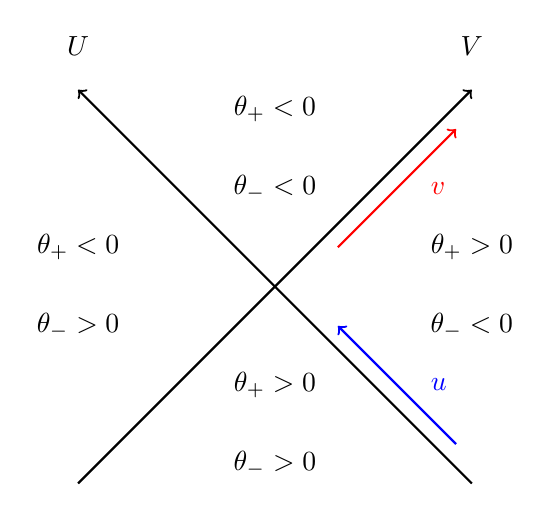
\begin{tikzpicture}

\draw[thick, ->] (-2.5,-2.5) -- node[at end, above=0.3cm]{$V$} (2.5,2.5);
\draw[thick, ->] (2.5,-2.5) -- node[at end, above=0.3cm]{$U$} (-2.5,2.5);

\node (a) at (2.5,0.5) {$\theta_+ > 0$};
\node (a) at (2.5,-0.5) {$\theta_- < 0$};

\node (a) at (-2.5,0.5) {$\theta_+ < 0$};
\node (a) at (-2.5,-0.5) {$\theta_- > 0$};

\node (a) at (0,2.25) {$\theta_+ < 0$};
\node (a) at (0,1.25) {$\theta_- < 0$};

\node (a) at (0,-1.25) {$\theta_+ > 0$};
\node (a) at (0,-2.25) {$\theta_- > 0$};

%\node (0) at (-3, -3) {$\theta_+ = 0$};
%\node (0) at (3, -3) {$\theta_- = 0$};

\draw[thick, ->, red] (0.8,0.5) -- node[midway, right=0.3cm] {$v$} (2.3,2) ;
\draw[thick, ->, blue] (2.3,-2) -- node[midway, right=0.3cm] {$u$} (0.8, -0.5);

\end{tikzpicture}
\caption[Signs of the expansions $\theta_\pm$ in the four quadrants of the Kruskal diagram for the Schwarzschild solution]{Signs of the expansions $\theta_\pm$ in the four quadrants of the Kruskal diagram of the \sch solution. The red arrow is outwards pointing and flows with increasing $v$, the blue arrow is inwards pointing and flows with increasing $u$.}
\label{fig:expansions}
\end{figure}

\subsection{Penrose-Carter diagram}

The Kruskal coordinates of the \sch solution give a representation for the global structure of the spacetime. We are able to plot the horizons, singularities and surfaces of constant coordinates, but the asymptotic region built of the `points at infinity' can't be included into the Kruskal diagram. 

The aim of a Penrose-Carter diagram is to compactify the spacetime in such a way that points at infinity are mapped to a finite point while maintaining the lightcone structure of the spacetime. To do this, we make a conformal transformation of the metric $\bar{g} = \Omega^2 g$, where $\Omega$ is a smooth function defined in the spacetime $M$. This new metric $\bar{g}$ allows the extension from $(M, \bar{g})$ to a larger, unphysical spacetime $\bar{M}$. To bring infinity to constant values, we require that $\Omega \rightarrow 0$ in the asymptotic limit; we can then understand the physical spacetime $M$ in $\bar{M}$ with a boundary $\partial M$ for $\Omega = 0$. In the following discussion, we perform this transformation on Minkowski spacetime as an example and then proceed to the \sch solution. 

\subsubsection{Minkowski spacetime}

Using ingoing and outgoing null coordinates
\begin{equation*}
	v = t + r, \qquad u = t - r, \qquad - \infty < u \leq v < \infty,
\end{equation*}
we can write down the Minkowski solution as
\begin{equation*}
	g = - du dv + \frac14 \left(v - u \right)^2 \left(d\theta^2 + \sin^2 \theta d\phi^2 \right).
\end{equation*}
The aim now is to make a coordinate transformation such that the range of the null coordinates is finite. We can do this using the transformation
\begin{equation*}
	u = \tan x, \qquad v = \tan y, \qquad -\frac{\pi}{2} < x \leq y < \frac{\pi}{2},
\end{equation*}
such that the metric is in the form
\begin{equation*}
	g = \left(2\cos x \cos y \right)^{-2} \left[ -4 dx dy + \sin^2(y - x) \left(d\theta^2 + \sin^2 \theta d\phi^2 \right) \right] .
\end{equation*}
Notice that in this form, all our coordinates have a finite range and that there is a conformal factor in the metric. By picking $\Omega = 2\cos x \cos y$, we can write down
\begin{equation*}
	\bar{g} = \Omega^2 g =  -4 dx dy + \sin^2(y - x) \left(d\theta^2 + \sin^2 \theta d\phi^2 \right) .
\end{equation*}
We now perform the coordinate transformation
\begin{equation*}
	T = x + y \in (-\pi, \pi), \qquad R = y - x \in [0, \pi),
\end{equation*}
such that the metric is of the form
\begin{equation*}
	\bar{g} = - dT^2 + dR^2 + \sin^2 R \left(d\theta^2 + \sin^2 \theta d\phi^2 \right).
\end{equation*}
In this form, we understand the metric $\bar{g}$ having the topology $I \times S^3$ for the interval $T \in I = (-\pi, \pi)$. If instead we had $T \in \mathbb{R}$, the above metric would be the Einstein static universe with the topology $\Real \times S^3$ \cite{Wald:106274}. We understand $\bar{g}$ as a section of the Einstein static universe for bounded $T$. 

Plotting the spacetime above onto the $(T,R)$ plane, we obtain the Penrose-Carter diagram for Minkowski space (Figure \ref{fig:minkpenrose}) where each point on the diagram represents a two-sphere. The boundary of the diagram corresponds to either $r = 0$, or to the points at infinity.

To understand the `infinite distance' points, we can study the radial geodesics of the spacetime. Radial null geodesics are the null curves of the flat metric $ds^2 = -dT^2 + dR^2$ and so run as straight lines at an angle of $45^\circ$. These null curves originate from the null surface $\scri^-$ (given by a surface of constant $T - R$) pass through the origin for $r = 0$ and end at the null surface $\scri^+$, given by a surface of constant $T + R$. We refer to  $\scri^+$ as \emph{future null infinity} and $\scri^-$ as \emph{past null infinity}. All timelike geodesics originate from the point $i^-$ and end at $i^+$ which are named \emph{past timelike infinity} and \emph{future timelike infinity} respectively. We see that these points are located for $(T,R) = (\pm \pi, 0)$ on the Penrose-Carter diagram, and are therefore the points $(u,v) = (\pm \infty, \pm \infty)$ written in terms of the original null coordinates for the metric $g$. Finally, all spacelike curves originate from the point $i^0$, which we refer to as \emph{spatial infinity} located for $(T,R) = (0,\pi)$, or $(u,v) = (-\infty, \infty)$. 

\begin{figure}[!h]
\centering
\begin{tikzpicture}
\node (I)    at (3,0)   {};

\draw [white!30!black] (3,-3) edge[bend right=40,looseness=2] (3,3);
\draw [white!30!black] (3,-3) edge[bend right=40,looseness=1.5] (3,3);
\draw [white!30!black] (3,-3) edge[bend right=40,looseness=1] (3,3);
\draw [white!30!black] (3,-3) edge[bend right=40,looseness=0.5] (3,3);

\draw [white!30!black] (3,0.75) parabola (6,0);
\draw [white!30!black] (3,-0.75) parabola (6,0);
\draw [white!30!black] (3,1.5) parabola (6,0);
\draw [white!30!black] (3,-1.5) parabola (6,0);


\draw[thick, blue, ->-] (4.5, -1.5) -- (3,0);
\draw[thick, red, ->-]  (3,0) -- (4.5, 1.5);

\path
   (I) +(90:3)  coordinate[label=45:$i^+$] (Itop)
       +(-90:3) coordinate[label=-45:$i^-$] (Ibot)
       +(0:3)   coordinate[label=45:$i^0$] (Iright)
       ;

\draw (Itop) -- 
      (Ibot) --
          node[midway, below right] {$\cal{J}^-$} 
      (Iright) -- 
          node[midway, above right] {$\cal{J}^+$} 
      (Itop) -- cycle;

\draw[->, white!50!black] (3,0) -- (6.5,0) node[right, black] {$R$};
\draw[->, white!50!black] (3,-3) -- node[above, sloped, black] {$r = 0 \quad $} (3,3.5) node[left, black] {$T$};

\node at (3,3) [circle,fill,inner sep=1.2pt]{};
\node at (6,0) [circle,fill,inner sep=1.2pt]{};
\node at (3,-3) [circle,fill,inner sep=1.2pt]{};


\end{tikzpicture}
\caption[Penrose-Carter diagram for Minkowski spacetime.]{Penrose-Carter diagram for Minkowski spacetime. The points $i^\pm$ are future (past) timelike infinity, at the points $(T,R) = (\pm \pi, 0)$, $i^0$ is spacial infinity at the point $(T,R) = (0,\pi)$ and $\scri^{\pm}$ are future (past) null infinity and are the null surfaces for surfaces of constant $T \pm R$.}
\label{fig:minkpenrose}
\end{figure}


\subsubsection{Kruskal spacetime}

We can carry out the same kind of coordinate transformation on the metric \eq{krusmet} to `compactify' the Kruskal diagram to obtain the Penrose-Carter diagram for the \sch solution. It is possible to do this carefully with a set of coordinate transformations as we have done previously; luckily for us though, the explicit work isn't necessary. As the \sch solution is asymptotically flat, the structure of the boundary of the Penrose-Carter diagram for the \sch solution will be of the same form as the Minkowski diagram. As there are two copies of an asymptotic spacetime for the Kruskal spacetime, there will then be two distinct sets of infinite boundaries for the Penrose-Carter diagram.

Null geodesics will still be lines running at $45^\circ$, originating at $\scri^-$, only now we find that not all null geodesics will terminate at $\scri^+$. Future-directed null geodesics which pass through the event horizon will inevitably fall to the singularity at $r = 0$. Conventionally, the conformal factor $\Omega$ used the set the asymptotic boundary is also picked such that the singularity $r = 0$ is represented as a horizontal line. As this point is not within our spacetime, it is represented by a wavey line in the diagram. Timelike geodesics still originate from $i^-$, but as with the null geodesics, only those which do not pass the event horizon will end at $i^+$. This same story is repeated under time reversal. All causal geodesics will end at $\scri^+$ or $i^+$, but the contribution to these points will come from $\scri^-$ and $i^-$, or from the white hole horizon.

Putting this all together, we can draw the Penrose-Carter diagram for the \sch solution, shown in Figure \ref{fig:penrosesch}. We note that this method of constructing the Penrose-Carter diagram piece by piece and comparing with known structures, is how the diagrams are conventionally built. We will apply this same method in Section \ref{sec:rnsol}, as well as in our novel solutions in Chapter \ref{ch:planarem} and Chapter \ref{ch:planarstu}.

\begin{figure}[!h]
\centering
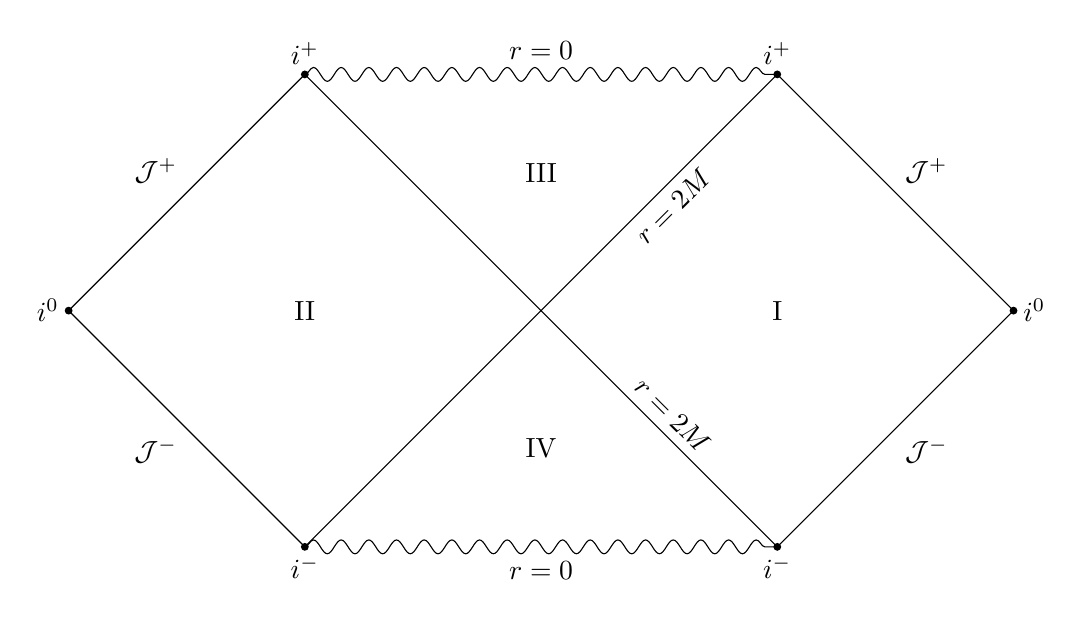
\begin{tikzpicture}
\node (I)    at ( 3,0)   {I};
\node (II)   at (-3,0)   {II};
\node (III)  at (0, 1.75) {III};
\node (IV)   at (0,-1.75) {IV};

\path  % Four corners of left diamond
  (II) +(90:3)  coordinate[label=90:$i^+$]  (IItop)
       +(-90:3) coordinate[label=-90:$i^-$] (IIbot)
       +(0:3)   coordinate                  (IIright)
       +(180:3) coordinate[label=180:$i^0$] (IIleft)
       ;
\draw (IIleft) -- 
          node[midway, above left]    {$\cal{J}^+$}
          node[midway, below, sloped] {$$}
      (IItop) --
          node[midway, below, sloped] {$$}
      (IIright) -- 
          node[midway, below, sloped] {$$}
      (IIbot) --
          node[midway, above, sloped] {$$}
          node[midway, below left]    {$\cal{J}^-$}    
      (IIleft) -- cycle;

\path % Four conners of the right diamond (no labels this time)
   (I) +(90:3)  coordinate[label=90:$i^+$] (Itop)
       +(-90:3) coordinate[label=-90:$i^-$] (Ibot)
       +(180:3) coordinate (Ileft)
       +(0:3)   coordinate[label=0:$i^0$] (Iright)
       ;
% No text this time in the next diagram
\draw (Ileft) -- 
          node[midway, below, sloped] {$r = 2M$}
      (Itop) --
          node[midway, above right] {$\cal{J}^+$} 
      (Iright) -- 
          node[midway, below right] {$\cal{J}^-$} 
      (Ibot) --
          node[midway, above, sloped] {$r = 2M$}   
      (Ileft) -- cycle;

% Squiggly lines
\draw[decorate,decoration=snake] (IItop) -- (Itop)
      node[midway, above, inner sep=1.8mm] {$r=0$};

\draw[decorate,decoration=snake] (IIbot) -- (Ibot)
      node[midway, below, inner sep=1.8mm] {$r=0$};

\node at (3,3) [circle,fill,inner sep=1pt]{};
\node at (6,0) [circle,fill,inner sep=1pt]{};
\node at (3,-3) [circle,fill,inner sep=1pt]{};
\node at (-3,3) [circle,fill,inner sep=1pt]{};
\node at (-6,0) [circle,fill,inner sep=1pt]{};
\node at (-3,-3) [circle,fill,inner sep=1pt]{};

\end{tikzpicture}
\caption[Penrose-Carter diagram for the Schwarzschild solution]{Penrose-Carter diagram for the Schwarzschild solution.}
\label{fig:penrosesch}
\end{figure}

\subsection{Asymptotic flatness}
\label{sec:asymptoticflatness}

Leading to this point, we have mentioned that the \sch solution is asymptotically flat, with the understanding that at an infinite distance, the manifold $(M,g)$ looks like the Minkowski spacetime. Here we discuss this in a bit more detail.

A common way to study systems is by assuming that they are isolated. By understanding Minkowski space as the background of a solution, we can think of asymptotic flatness as the statement that from an infinite distance from a source, spacetime appears to be empty. 

In this thesis, we consider planar symmetric solutions to the field equations, and for all the solutions we derive, we find that the solutions are not asymptotically flat. Asymptotic flatness is a key assumption for the derivation of many quantities in black hole physics. In a sense, we can understand the existence of an asymptotically flat region to the solution as giving us a natural background to work from.

From the perspective of the metric tensor, we say that the spacetime is asymptotically flat if there exists a system of coordinates $\{t,x,y,z\}$, where $r^2 = x^2 + y^2 + z^2$ such that the metric tensor can be written as
\begin{equation*}
	g_{\mu \nu} = \eta_{\mu \nu} + h_{\mu \nu}(x^\mu),
\end{equation*}
and the tensor $h_{\mu \nu}$ depends on $r$ in the following ways
\begin{equation*}
\begin{aligned}
	&\lim_{r \rightarrow \infty} h_{\mu \nu}(x^\mu) & &\rightarrow \quad \Op(r^{-1}), \\
	&\lim_{r \rightarrow \infty} h_{\mu \nu, \rho}(x^\mu) & &\rightarrow \quad \Op(r^{-2}) ,\\
	&\lim_{r \rightarrow \infty} h_{\mu \nu, \rho \sigma}(x^\mu) & &\rightarrow \quad \Op(r^{-3}).
\end{aligned}
\end{equation*}
However, this coordinate-dependent method to identify asymptotically flat spacetimes is difficult to work with in general. This method will be enough for our work, but we note that the best way to classify asymptotically flat spacetimes is by showing that the structure of null infinity $\scri^\pm$ is the same as for the Minkowski solution. More details on this are given in \cite{Hawking:1973uf, Wald:106274}.

\section{Reissner-Nordstr\"om solution}
\label{sec:rnsol}
\subsection{Solving the equations of motion}

In this section, we derive the static, spherically symmetric solution to Einstein-Maxwell theory to produce a charged black hole known as the \emph{Reissner-Nordstr\"om} solution. The action for Einstein-Maxwell theory is given by
\begin{equation}
\label{eq:EMaction}
	S = \frac{1}{16\pi} \int d^4x \sqrt{-g} (-R - F^2).
\end{equation}
Where $F = dA$ is the 2-form field strength. We note here that we adopt the relativistic convention for the gauge coupling which is $g = 4\pi$ and $G = 1$, chosen to unify the couplings from the Ricci and Maxwell terms. We will allow the black hole to be supported by both electric and magnetic charges. Einstein's equations are given by
\begin{equation*}
   R_{\mu \nu} - \half g_{\mu\nu} R = - \left( F_{\mu \rho} \tensor{F}{_\nu^{\rho}} - \frac{1}{4} g_{\mu \nu} F_{\rho \sigma} F^{\rho \sigma} \right),
\end{equation*}
where we have used that the energy-momentum tensor is
\begin{equation}
\label{eq:rnstressenergy}
   T_{\mu \nu} = -\frac{2}{\sqrt{-g}} \frac{ \delta S_{M}}{\delta g^{\mu \nu}} =  \frac{1}{8\pi} \left( F_{\mu \rho} \tensor{F}{_\nu^{\rho}} - \frac{1}{4} g_{\mu \nu} F_{\rho \sigma} F^{\rho \sigma} \right).
\end{equation}
Using that $T_{\mu \nu}$ is traceless, we can rewrite Einstein's equations as
\begin{equation}
\label{eq:rnee}
   R_{\mu \nu} = -8 \pi T_{\mu \nu},
\end{equation}
and Maxwell equations are 
\begin{equation*}
   \nabla_\mu F^{\mu \nu} = 0, \qquad \nabla_{[\mu} F_{\nu \rho]} = 0.
\end{equation*}
We begin our solution by writing down a metric ansatz compatible with a stationary, spherically symmetric spacetime
\begin{equation*}
   ds^2 = -e^{2F(r,t)} dt^2 + e^{2H(r,t)} dr^2 + r^2(d\theta^2 + \sin^2 \theta d\phi^2),
\end{equation*}
where the timelike direction $t$, is orthogonal to all spacelike directions. Considering the electromagnetic field strength, our assumption of spherical symmetry results in the only non-zero field components being the radial ones. For the electric field we have
\begin{equation*}
   E_r = F_{tr} = -F_{rt} = \alpha(t,r),
\end{equation*}
and for the magnetic field we use
\begin{equation*}
\begin{aligned}
     B_\mu = g_{\mu \nu} \et^{t \nu \rho \sigma} F_{\rho \sigma},
\end{aligned}
\end{equation*}
to write down the form of the radial component of the magnetic field
\begin{equation*}
   B_r = \frac{2g_{rr}}{r^2 \sin \theta} F_{\theta \phi}.
\end{equation*}
For $B_r$ to have no $\theta$ component, the field strength must be of the form\footnote{Note here that the explicit $r^2$ term appears for cosmetic reasons which become apparent in the following calculations.}
\begin{equation*}
    F_{\theta \phi} = \beta(t,r) r^2 \sin \theta,
\end{equation*}
which we can use to write down the most general field strength tensor for a spherically symmetric solution
\begin{equation*}
   F_{\mu \nu} = \begin{pmatrix} 0 & \alpha(t,r) & 0 & 0 \\ -\alpha(t,r) & 0 & 0 & 0 \\ 0 & 0 & 0 & \beta(t,r) r^2 \sin \theta \\ 0 & 0 & -\beta(t,r) r^2 \sin \theta & 0 \end{pmatrix}.
\end{equation*}
From this and Equation \eq{rnstressenergy}, we compute the non-zero components of the energy-momentum tensor
\begin{equation}
\label{eq:rnemt}
   \begin{aligned}
     T_{tt} &= \frac{1}{8 \pi} \bigg(\alpha^2(t,r) e^{-2H} + \beta^2(t,r) e^{2F} \bigg),\\
     T_{rr} &= -\frac{1}{8 \pi}\bigg(\alpha^2(t,r) e^{-2F} + \beta^2(t,r) e^{2H} \bigg), \\
     T_{\theta \theta} &= \frac{r^2}{8 \pi} (\alpha^2 e^{-2(F+H)} + \beta^2),\\
     T_{\phi \phi} &=   T_{\theta \theta}\sin^2\theta.
   \end{aligned}
\end{equation}

We now turn our attention to calculating the components of the Ricci scalar. Using \eq{chs}, and the components of the inverse metric
\begin{equation*}
	g^{\mu \nu} = \fourdiagmat{-e^{-2F(t,r)}}{e^{-2H(t,r)}}{r^{-2}}{r^{-2} \sin^{-2}\theta},
\end{equation*}
the non-zero values of \eq{chs} are
\begin{equation*}
   \begin{aligned}
    &\tensor{\Gamma}{^{t}_{tt}} = \partial_t F(t,r), \quad &&\tensor{\Gamma}{^{t}_{tr}} = \partial_r F(t,r) , \quad &&&&\tensor{\Gamma}{^{t}_{rr}} = e^{2(H-F)}\partial_t H(t,r) , \\
    &\tensor{\Gamma}{^{r}_{tt}} = e^{2(F-H)}\partial_r F(t,r)  ,\quad &&\tensor{\Gamma}{^{r}_{tr}} = \partial_t H(t,r) , \quad &&&&\tensor{\Gamma}{^{r}_{rr}} =  \partial_r H(t,r) , \\
    &\tensor{\Gamma}{^{r}_{\theta \theta}} = -re^{-2H} ,\quad &&\tensor{\Gamma}{^{r}_{\phi \phi}} = -r\sin^2\theta e^{-2H}, \quad &&&&\tensor{\Gamma}{^{\theta}_{r \theta}} = \frac{1}{r} ,\\
    &\tensor{\Gamma}{^{\theta}_{ \phi \phi}} = -\cos \theta \sin \theta ,\quad &&\tensor{\Gamma}{^{\phi}_{r \phi}} = \frac{1}{r} ,\quad &&&&\tensor{\Gamma}{^{\phi}_{\theta \phi}} = \cot \theta .\\
   \end{aligned}
\end{equation*}
The Riemann tensor expressed in terms of the Christoffel symbols is given in \eq{riemannchs} and when contracted yields the expression for the Ricci tensor
\begin{equation}
\label{eq:ricchs}
   R_{\mu \nu} = \tensor{R}{^{\lambda}_{\mu \lambda \nu}} = -\left(\partial_\lambda \tensor{\Gamma}{^{\lambda}_{\mu \nu}} - \partial_\nu \tensor{\Gamma}{^{\lambda}_{\mu \lambda}} + \tensor{\Gamma}{^{\lambda}_{\lambda \tau}}\tensor{\Gamma}{^{\tau}_{\mu \nu}} - \tensor{\Gamma}{^{\lambda}_{\nu \tau}}\tensor{\Gamma}{^{\tau}_{\mu \lambda}} \right).
\end{equation}
 Substituting in the values for the Christoffel symbols, the non-zero components of the Ricci tensor are found to be
 \begin{equation}
   \begin{aligned}
   R_{tt} &= -e^{2(F-H)}\bigg(\pardev{F}{r} \bigg( \pardev{F}{r} - \pardev{H}{r} +\frac{2}{r} \bigg) + \pardev{^2 F}{r^2} \bigg) - \pardev{H}{t} \bigg( \pardev{F}{t} - \pardev{H}{t} \bigg) - \pardev{^2 H}{t^2}, \\  
   R_{rr} &= -e^{2(H-F)} \bigg(\pardev{^2H}{t^2} + \pardev{H}{t}\bigg(\pardev{H}{t}-\pardev{F}{t} \bigg)\bigg) - \pardev{F}{r} \bigg(\pardev{H}{r} + \pardev{F}{r} \bigg) + \pardev{^2 F}{r^2} - \frac{2}{r} \pardev{H}{r} ,\\
   R_{\theta \theta} &= e^{-2H} \left( r\pardev{F}{r} - r\pardev{H}{r} + 1 \right) + 1 ,\\
   R_{\phi \phi} &= R_{\theta \theta} \sin^2\theta  ,\\
    R_{tr} &= - \frac{2}{r} \pardev{H}{t}.
   \end{aligned}
\end{equation}
With \eq{rnee} and that $T_{tr} = 0$, we can deduce that
\begin{equation*}
	R_{tr} = \frac{2}{r} \pardev{H}{t} = 0, \quad \Rightarrow \quad H(r,t) = h(r).
\end{equation*}
Adding components from \eq{rnemt} we find that
\begin{equation*}
   \begin{aligned}
     T_{rr} + e^{2(h-F)}T_{tt} = 0,
   \end{aligned}
\end{equation*}
which when substituted into \eq{rnee}, we obtain
\begin{equation*}
	R_{rr} +  e^{2(h-F)} R_{tt} = \frac{2}{r} \left( \pardev{F}{r} - \pardev{h}{r} \right) = 0.
\end{equation*}
This allows us to pull apart the functional dependence of $F(t,r)$ and find
\begin{equation*}
	\pardev{F}{r} - \pardev{h}{r} = 0 \quad \Rightarrow \quad F(r,t) = g(t) - h(r).
\end{equation*}
Through redefinition of the coordinate $t$, we can absorb $g(t)$ such that $F(t,r) = f(r) = -h(r)$ and the line element for our solution takes the form
\begin{equation*}
   ds^2 = -e^{2f(r)} dt^2 + e^{-2f(r)} dr^2 + r^2 d\Omega^2.
\end{equation*}
Before continuing, we note here that through the assumption that our solution is spherically symmetric and stationary, we obtain a static line element with no extra assumptions.

The last differential equation to solve is
\begin{equation}
\label{eq:lbit}
    R_{\theta \theta} = -8 \pi T_{\theta \theta},
\end{equation}
but before we do this, let's look at the Maxwell equations to determine the exact form of the functions $\alpha(t,r)$ and $\beta(t,r)$.
 
Maxwell's equations can be simplified using the identity
\begin{equation*}
\begin{aligned}
     \nabla_\mu F^{\mu \nu} &= \frac{1}{\sqrt{|g|}} \partial_\mu (\sqrt{|g|} F^{\mu \nu}), \\
     &= \frac{1}{r^2\sin \theta} \partial_\mu (r^2\sin \theta F^{\mu \nu}).
\end{aligned}
\end{equation*}
In particular, if we look at the $r$-component we obtain
\begin{equation}
   \partial_t F_{tr} = 0 \quad \Rightarrow \quad \alpha(t,r) = \alpha(r).
\end{equation}
For the $t$-component of the equation we obtain:
\begin{equation*}
   \partial_r (r^2 F^{rt}) = \partial_r (g^{tt}g^{rr}F_{tr}) = 0 \quad \Rightarrow \quad \alpha(r) = \frac{C}{r^2}.
\end{equation*}
We can fix the value of the constant using Gauss' law. Doing this we find
\begin{equation*}
   \alpha(r) =\frac{Q}{r^2},
\end{equation*}
where $Q$ is the total electric charge of the black hole.
 
To obtain the form for $\beta(t,r)$, we use the Bianchi identity
\begin{equation*}
   \nabla_{\mu} F_{\nu \rho} + \nabla_{\nu} F_{\rho \mu} +\nabla_{\rho} F_{\mu \nu} = 0.
\end{equation*}
When the connections are expanded in terms of Christoffel symbols, we find we are left only with partial derivatives
\begin{equation*}
   \partial_{\mu} F_{\nu \rho} + \partial_{\nu} F_{\rho \mu} +\partial_{\rho} F_{\mu \nu} = 0.
\end{equation*}
Choosing our indices such that $\mu = t$, $\nu = \phi$ and $\rho = \theta$ we find
\begin{equation*}
   \partial_t F_{\theta \phi} = 0 \quad \Rightarrow \quad \beta(t,r) = \beta(r).
\end{equation*}
If we instead pick $\mu = r$, $\nu = \theta$ and $\rho = \phi$, we obtain the differential equation
\begin{equation*}
    \partial_r (r^2 \beta) = 0 \quad \Rightarrow \quad \beta(r) = \frac{P}{r^2},
\end{equation*}
where $P$ is the total magnetic charge of the black hole.
 
Turning our attention back to \eq{lbit} we find that:
\begin{equation*}
   \begin{aligned}
     R_{\theta \theta} &= \partial_r (re^{2f}) - 1=  -8 \pi  T_{\theta \theta} , \\
     &\Rightarrow \partial_r (re^{2f}) = 1 - 8 \pi \frac{r^2}{8 \pi r^4} (Q^2 + P^2) ,\\
     & \Rightarrow \partial_r (re^{2f}) = 1 - \frac{1}{r^2} (Q^2 + P^2).
   \end{aligned}
\end{equation*}
Integrating with respect to $r$, we obtain
\begin{equation}
\label{eq:rnsol}
   e^{2f(r)} = 1 - \frac{\mu}{r} + \frac{e^2}{r^2},
   \end{equation}
where $e = \sqrt{Q^2 + P^2}$ is the total charge. To set the final integration constant $\mu$, we can take the limit in which the charges tend to zero and compare our result with Newtonian gravity by taking the weak field approximation
\begin{equation}
\label{eq:weakle}
   ds^2 = -\left(1+\frac{\mu}{r}\right)dt^2 + \left(1+\frac{\mu}{r}\right)^{-1} dr^2 + r^2 d\Omega^2.
\end{equation}
The line element for Newtonian gravity is known \cite{Wald:106274}
\begin{equation}
\label{eq:newtle}
   ds^2 = -(1 + 2\Phi) dt^2 + (1 - 2\Phi)dr^2 + r^2 d\Omega^2,
\end{equation}
where the gravitational potential $\Phi$ is given by\footnote{We reiterate that we are working in natural units where Newton's constant $G=1$.}
\begin{equation*}
    \Phi = -\frac{M}{r}.
\end{equation*}
By comparing \eq{newtle} with \eq{weakle} we can identify
\begin{equation*}
   \mu = -2M,
\end{equation*}
where $M$ is the mass of the black hole. Substituting this into \eq{rnsol} we obtain the \emph{Reissner-Nordstr\"om} solution
\begin{equation}
\label{eq:rnsolfull}
\begin{aligned}
  ds^2 &=  -\left( 1 - \frac{2M}{r} + \frac{e^2}{r^2} \right) dt^2 + \left( 1 - \frac{2M}{r} + \frac{e^2}{r^2} \right)^{-1} dr^2 + r^2 d\Omega^2	, \\
  A &= - \frac{Q}{r} dt - P \cos \theta d\phi, \quad e = \sqrt{Q^2 + P^2},
\end{aligned}
\end{equation}
where $A$ is the gauge potential from which we obtain the field strength $F = dA$. The solution \eq{rnsolfull} is the general solution of the coupled Maxwell-Einstein equations for a spherically symmetric spacetime, and can be proven as the unique solution with a generalisation of Birkhoff's theorem \cite{Ellis:2013dla}. The Reissner-Nordstr\"om solution is parametrised by three constants: the mass $M$, the electric charge $Q$ and magnetic charge $P$. 

In Section \ref{sec:gravitationalmass} we will discuss in more detail how the mass parameter of a black hole solution can be derived, but for now we will use that the mass is exactly given by the parameter $M$. We can compute the conserved electric and magnetic charges of the black hole with the integrals
\begin{equation}
\label{eq:gausslawcharges}
	\mathcal{Q} = \lim_{r \rightarrow \infty} \frac{1}{4\pi} \int_{S^2} \star F, \qquad \mathcal{P} = \lim_{r \rightarrow \infty} \frac{1}{4\pi} \int_{S^2} F.
\end{equation}	
These integrals can be understood as the curved spacetime generalisation of Gauss' law. These integrals will pop up again and again throughout the thesis, but in Section \ref{sec:electromagneticduality} we consider Abelian gauge fields and their conserved charges. As an example, we can use the field strength computed from \eq{rnsolfull} and the Hodge-star to compute the conserved electric charge
\begin{equation}
\label{eq:rnelecharge}
	\begin{aligned}
		\mathcal{Q} &= \lim_{r \rightarrow \infty} \frac{1}{4\pi} \int_{S^2} \star F, \\
		&= \lim_{r \rightarrow \infty} \frac{1}{4\pi} \int g^{tt} g^{rr} F_{tr} r^2 \sin \theta d\theta d\phi, \\ 
		&= Q.
	\end{aligned}
\end{equation}
In a similar way, the magnetic charge is given by
\begin{equation}
\label{eq:rnmagcharge}
	\mathcal{P} = \lim_{r \rightarrow \infty} \frac{1}{4\pi} \int_{S^2} F = P.
\end{equation}

\subsection{Causal structure}
\label{sec:rncausal}

Unlike the \sch solution, we see the function
\begin{equation}
\label{eq:rnzeros}
	f(r) = \left( 1 - \frac{2M}{r} + \frac{e^2}{r^2} \right) = \frac{(r - r_+)(r - r_-)}{r^2}, \qquad r_{\pm} = M \pm \sqrt{M^2 - e^2},
\end{equation}
will have two zeros, provided that $M > e$. For the case with $M  = e$, there will be a single repeated zero for $r = M$. This solution is known as the \emph{extremal solution} and will be further discussed in Section \ref{sec:rnext}. For the case of $M < e$, there are no zeros for \eq{rnzeros} in the domain $r > 0$. The Kretschemann scalar for the Reissner-Nordstr\"om solution is given by \cite{Henry:1999rm}
\begin{equation*}
	K = R^{\mu \nu \rho \sigma} R_{\mu \nu \rho \sigma} = \frac{48M^2 r^2 - 96 M e^2 r+ 56 e^2}{r^8},
\end{equation*} 
which shows the presence of a curvature singularity for $r = 0$. We then understand the case for $M < e$ being a solution with a singularity without a horizon. These are known as \emph{naked singularities} and are generally deemed unphysical as they violate the cosmic censorship hypotheses.\footnote{The cosmic censorship hypotheses comes in two forms. The weak statement is that no singularities can be seen from future null infinity, and so must be hidden behind a horizon; this is what we will refer to by cosmic censorship in this thesis. The strong cosmic censorship hypothesis states that generically, the maximal Cauchy development of some initial dataset is inextendible. The strong cosmic censorship hypothesis -- despite the name -- does not  imply the weak version and Penrose's version \cite{Penrose:1969pc} of the strong version was disproven in \cite{Dafermos:2017dbw}.} As such, we will assume that $M \geq e$ for the following discussion. If one were to imagine a ball of matter with $M < e$, we would find the electromagnetic repulsion would prevent gravitational collapse. For quantum particles such as the electron with $Q > M$, we cannot employ these classical arguments.

The solution \eq{rnsolfull} derived from the Einstein-Maxwell action is well defined for $r > r_+$. The singularities for $r = r_\pm$ are coordinate singularities and it is possible to analytically continue through the horizons for $r = r_\pm$ with appropriate coordinate transformations to describe spacetime regions which extend from $0 < r < \infty$. 

We can perform an Eddington-Finkelstein transformation by identifying our tortoise coordinate
\begin{equation}
\label{eq:rntortoise}
	dr_\star = \frac{dr}{f(r)} \quad \Rightarrow \quad 	r_\star = r + \frac{1}{2 \kappa_+} \log \left| \frac{r - r_+}{r_+} \right| + \frac{1}{2 \kappa_-} \log \left| \frac{r - r_-}{r_-} \right|,
\end{equation}
with ingoing and outgoing null coordinates
\begin{equation*}
	v = t + r_\star, \qquad u = t - r_\star,
\end{equation*}
such that when expressed using ingoing coordinates the line element can be written as
\begin{equation*}
	ds^2 = - f(r) dv^2 + 2 dv dr_\star + r^2 d\Omega^2.
\end{equation*}
This line element is smooth for $r > 0$. 
In our Eddington-Finkelstein coordinates, the timelike Killing vector for $r > r_+$ is given by
\begin{equation*}
	k = \pardev{}{v}, \qquad k^\flat = -f(r) dv + dr, \qquad k^2 = -f(r).
\end{equation*} 
The null hypersurfaces located for $r = r_\pm$ are therefore Killing horizons. We denote the Killing horizon for $r = r_+$ as the \emph{outer horizon} and it can be shown that the region for $r < r_+$ is a black hole region with the event horizon located at $r = r_+$ \cite{Poisson:2009pwt}. The Killing horizon for $r = r_-$ is the inner horizon, and is formally known as a \emph{Cauchy horizon}. A Cauchy horizon is a null hypersurface which is also the boundary for the domain of validity of a Cauchy problem. Cauchy horizons are unstable \cite{Markovic:1994gy}, but as we will not be researching the stability of the Killing horizons we discuss in this thesis, we leave further discussion to the given references.  

In this coordinate system, we can compute the surface gravity \eq{surfacegravity} for the horizons located for $r = r_\pm$ and find that
\begin{equation}
\label{eq:rnsurfacegravity}
\begin{aligned}
		\kappa_\pm &= \half \partial_r f(r) \; \bigg|_{r = r\pm} \;, \\
	&= \frac{(r - r_+) + (r - r_-)}{2r^2} - \frac{(r - r_+)(r - r_-)}{r^3 } \bigg|_{r = r\pm} \; ,\\
	&= \frac{r_\pm - r_\mp}{2r_\pm^2}.
\end{aligned}
\end{equation}
Studying the line element given by the ingoing Eddington-Finkelstein coordinates, we see that the coordinates $(t,r)$ will be timelike/spacelike depending on the sign of the function $f(r)$. Starting in the region $r > r_+$, we can see that in the limit of $r \to \infty$, the line element \eq{rnsolfull} approaches the Minkowski solution. Crossing the event horizon at $r = r_+$, $f(r) < 0$, the coordinates $(t,r)$ are spacelike and timelike respectively. The region of spacetime between $r_+ > r > r_-$ is therefore time-dependent. The Cauchy horizon for $r = r_-$ is a point in time, which will eventually be crossed for all causal paths.\footnote{We can think of the inevitably of crossing $r = r_-$ in the same way that the curvature singularity is unavoidable for causal curves that cross $r = 2M$ in the \sch solution.} There is a physical singularity at $r = 0$, which is a point in space which can then be avoided.\footnote{This is in contrast to the spacelike singularity of the \sch solution which is a point of time and is thus reached for all causal geodesics within the black hole region.}

In Poisson's textbook \cite{Poisson:2009pwt}, the Kruskal coordinate system for the Reissner-Nordstr\"om solution is given great care. However, it is possible to construct the Penrose-Carter diagram for the spacetime patch-wise, based off the discussion above. The diagram is given in Figure \ref{fig:PenroseRN}, with a conformal factor picked such that the timelike singularities are depicted with a vertical wavey line. Thinking of some future-directed causal curve, one can follow the path of a geodesic which begins from $\scri^-$ in region VIII, moves through the event horizon into region III, and inevitably crosses the Cauchy horizon and reaches the region with a singularity in region IV. The regions VII and VIII are isomorphic, as are regions II and IV. Unlike the \sch solution though, the causal curve is not doomed to remain in the region containing the singularity and can cross the horizon at $r = r_-$ into region I, which is isomorphic to region III. Here, the horizon $r = r_+$ is a point in time and the causal curve must continue through into region V or VI, which are isomorphic not only with each other, but also to VII and VIII. We see that the causal path has traversed from one asymptotically flat patch into another one! We might think that this contradicts the assertion that the null hypersurface ar $r = r_+$ is an event horizon, seeing as the path has `escaped' but what we must consider is that the regions VIII and VI are distinct in that one cannot communicate between the regions. Once a causal path crosses the horizon in region VIII, it is impossible for it to reach $\scri^+$ in region VIII. 


\begin{figure}[p!]
\centering
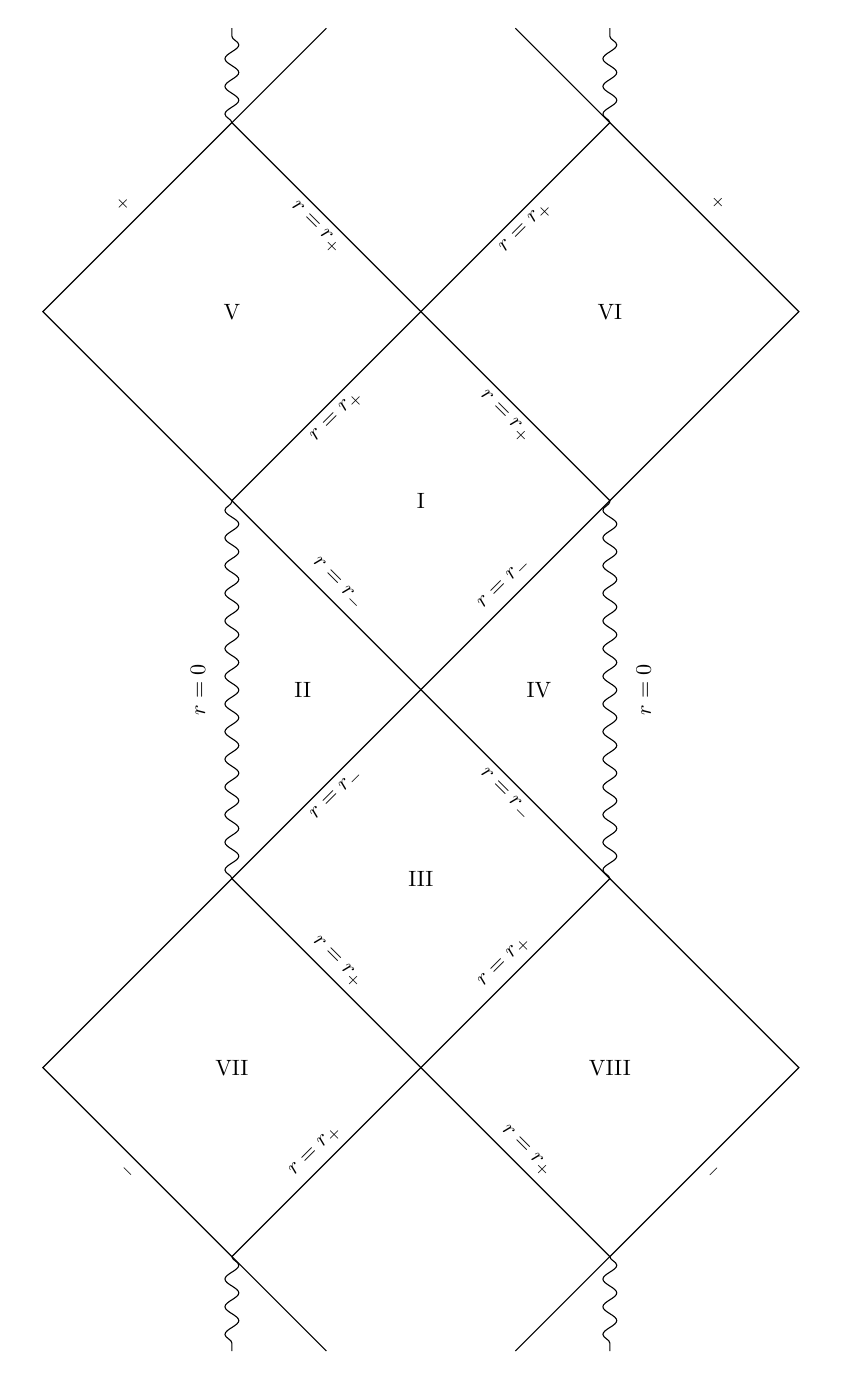
\begin{tikzpicture}[scale=0.6, every node/.style={scale=0.8}]
\node[above] (0) at (0.13,12) {};
\node[below] (1) at (0.13,-4) {};

\node (I) at (0,8) {I};
\node (II) at (0,0) {III};
\node (III) at (-2.5,4) {II};
\node (IV) at (2.5,4) {IV};

\node (V) at (-4,12) {V};
\node (VI) at (4,12) {VI};

\node (VII) at (-4,-4) {VII};
\node (VIII) at (4,-4) {VIII};

\path % Four corners of left diamond
 (I) +(90:4) coordinate[label=90:] (IItop)
 +(-90:4) coordinate(IIbot)
 +(0:4) coordinate[label=360:] (IIright)
 +(180:4) coordinate[label=180:] (IIleft)
 ;
\draw (IIleft) --
 node[midway, below, sloped] {$r = r_+$}
 (IItop) --
 node[midway, below, sloped] {$r = r_+$}
 (IIright)
     node[midway, above, sloped] {}
           --
 node[midway, above, sloped] {$r = r_-$}
 (IIbot) --
 node[midway, above, sloped] {$r = r_-$}
 (IIleft) -- cycle;


\path % Four conners of the right diamond (no labels this time)
 (II) +(90:4) coordinate (Itop)
 +(-90:4) coordinate (Ibot)
 +(180:4) coordinate (Ileft)
 +(0:4) coordinate (Iright)
 ;
% No text this time in the next diagram
\draw (Ileft) --
 node[midway, below, sloped] {$r = r_-$}
 (Itop) --
 node[midway, below, sloped] {$r = r_-$}
 (Iright) --
 node[midway, above, sloped] {$r = r_+$}
 (Ibot) --
 node[midway, above, sloped] {$r = r_+$}
 node[midway, below, sloped] {}
 (Ileft) -- cycle;

\path % Four corners of left diamond
 (V) +(90:4) coordinate[label=90:] (Vtop)
 +(-90:4) coordinate(Vbot)
 +(0:4) coordinate[label=360:] (Vright)
 +(180:4) coordinate[label=180:] (Vleft)
 ;
 \draw (Vbot) --
 node[midway, below, sloped] {}
 (Vleft) --
 node[midway, above, sloped] {$\scri^+$}
 (Vtop)
     node[midway, above, sloped] {}
           --
 node[midway, below, sloped] {$r = r_+$}
 (Vright);
 
 \path % Four corners of left diamond
 (VI) +(90:4) coordinate[label=90:] (VItop)
 +(-90:4) coordinate(VIbot)
 +(0:4) coordinate[label=360:] (VIright)
 +(180:4) coordinate[label=180:] (VIleft)
 ;
 \draw (VIleft) --
 node[midway, below, sloped] {$r = r_+$}
 (VItop) --
 node[midway, above, sloped] {$\scri^+$}
 (VIright)
     node[midway, above, sloped] {}
           --
 node[midway, below, sloped] {}
 (VIbot);
 
 
 \path % Four corners of left diamond
 (VII) +(90:4) coordinate[label=90:] (VIItop)
 +(-90:4) coordinate(VIIbot)
 +(0:4) coordinate[label=360:] (VIIright)
 +(180:4) coordinate[label=180:] (VIIleft)
 ;
 \draw (VIItop) --
 node[midway, below, sloped] {}
 (VIIleft) --
 node[midway, below, sloped] {$\scri^-$}
 (VIIbot)
     node[midway, above, sloped] {}
           --
 node[midway, above, sloped] {$r = r_+$}
 (VIIright);
 
 \path % Four corners of left diamond
 (VIII) +(90:4) coordinate[label=90:] (VIIItop)
 +(-90:4) coordinate(VIIIbot)
 +(0:4) coordinate[label=360:] (VIIIright)
 +(180:4) coordinate[label=180:] (VIIIleft)
 ;
 \draw (VIIItop) --
 node[midway, below, sloped] {}
 (VIIIright) --
 node[midway, below, sloped] {$\scri^-$}
 (VIIIbot)
     node[midway, above, sloped] {}
           --
 node[midway, above, sloped] {$r = r_+$}
 (VIIIleft);


%Squiggly lines
\draw[decorate,decoration=snake,draw=black] (Ileft) -- (IIleft)
 node[midway, above=0.3cm, sloped] {$r = 0$};

\draw[decorate,decoration=snake, draw=black] (Iright) -- (IIright)
 node[midway, below=0.3cm, sloped] {$r = 0$};
 
 % cut off top
 \draw[decorate,decoration=snake, draw=black] (-4,16) -- (-4,18)
 node[midway, below, sloped] {};
  \draw[decorate,decoration=snake, draw=black] (4,16) -- (4,18)
 node[midway, below, sloped] {};
  \draw (-4,16) -- (-2,18)
 node[midway, below, sloped] {};
   \draw (4,16) -- (2,18)
 node[midway, below, sloped] {};
 
  % cut off bottom
 \draw[decorate,decoration=snake, draw=black] (-4,-8) -- (-4,-10)
 node[midway, below, sloped] {};
  \draw[decorate,decoration=snake, draw=black] (4,-8) -- (4,-10)
 node[midway, below, sloped] {};
  \draw (-4,-8) -- (-2,-10)
 node[midway, below, sloped] {};
   \draw (4,-8) -- (2,-10)
 node[midway, below, sloped] {};

%\draw[blue,dashed,bend right=25, thick] (Ileft) to (Iright);
%\draw[blue,dashed,bend right=-25, thick] (Ileft) to (Iright);
%\draw[blue,dashed,bend right=25, thick] (IIleft) to (IIright);
%\draw[blue,dashed,bend right=-25, thick] (IIleft) to (IIright);
%\draw[blue,dashed,bend right=25, thick] (Ileft) to (IIleft);
%\draw[blue,dashed,bend right=-25, thick] (Iright) to (IIright);
%\draw[->-,orange,bend right=-20, thick] (1) to (0);
\end{tikzpicture}
\caption[Penrose-Carter diagram for Reissner-Nordstr\"om solution]{Segment of the Penrose-Carter diagram for Reissner-Nordstr\"om solution. New patches can be reached in an infinite stack from above and below the diagram.}
\label{fig:PenroseRN}
\end{figure}

\subsection{Extremal solution}
\label{sec:rnext}

For the special case of $M = e$, the solution is said to be \emph{extremal}. The line element for the extremal Reissner-Nordstr\"om solution is given by
\begin{equation}
\label{eq:ernle}
	ds^2 = - \left(1 - \frac{M}{r} \right)^2 dt^2 + \left(1 - \frac{M}{r} \right)^{-2} dr^2 + r^2 d\Omega^2,
\end{equation}
where for $r > M$, the spacetime is static and the hypersurface for $r = M$ is a Cauchy horizon. The singularity at $r = M$ is a coordinate singularity, and by computing the Kretschmann Scalar
\begin{equation*}
	K = R^{\mu \nu \rho \sigma} R_{\mu \nu \rho \sigma} = \frac{8M^2 (7M^2 - 12MR+ 6r^2) }{r^8},
\end{equation*} 
we can identify $r = 0$ as a physical singularity.  

We may analytically continue the line element through making the coordinate transformation
\begin{equation*}
	r_* = r + 2M \log \left| \frac{r - M}{M} \right| - \frac{M^2}{r - M},
\end{equation*}
and introducing an ingoing Eddington–Finkelstein coordinate $v = t + r_*$. From this, we can write down a line element which extends past $r < M$ towards the singularity at $r=0$
\begin{equation*}
	ds^2 = - \left(1 - \frac{M}{r} \right)^2 dv^2 + 2 dv dr + r^2 d\Omega^2.
\end{equation*}
The extremal solution has an interesting behaviour for surfaces of constant $t$. Unlike Schwarzschild, where a surface of constant time is an Einstein-Rosen bridge connecting two spacetime regions, a surface of constant $t$ is an infinite throat. This can be seen by calculating the proper distance from a point $x > M$ to $M + \epsilon$:
\begin{equation*}
	s = \int^x_{M+\epsilon} \frac{r dr}{r - M} = \left[ M \log (r-M)+r \; \right]_{M+\epsilon}^x,
\end{equation*} 
which diverges as $\epsilon \rightarrow 0$. Looking more closely at the near horizon metric, we can understand this better. For $r = M(1 + \epsilon)$, the metric \eq{ernle} can be expanded for $\epsilon << 1$ and we find 
\begin{equation*}
	ds^2 = - \epsilon^2 dt^2 + \frac{M^2}{\epsilon^2} d\epsilon^2 + M^2 d\Omega^2.
\end{equation*}
This is the \emph{Robinson-Bertotti} metric, which is isometric to $AdS_2 \times S^2$. 

As with the non-extremal solution, the singularity is timelike and so avoidable for causal paths. We can think of the extremal solution as the limit where both horizons for $r = r_\pm$ coincide, and the time-dependent region of the spacetime is lost. In the extremal Reissner-Nordstr\"om solution, an observer in region I has two choices. It can either follow a causal path towards $\scri^+$, or it may cross the Cauchy horizon at $r = M$. After crossing the horizon, unlike in the \sch solution, the spacetime region remains static. This is because the coordinate $r$ remains spacelike throughout the geometry as $f(r) \geq 0$ for all $r$. The singularity is located for $r = 0$, which is simply a point in space and can be avoided. The causal observer can then continue through the horizon at $r = M$ into a new, asymptotically flat spacetime (region I$^\prime$). See Figure \ref{fig:PenroseERN}, for an illustration.

We can see that the area of the black hole is finite: $A = 4\pi r_h^2 = 4\pi M^2$, but if we compute the surface gravity on the Killing horizon using \eq{surfacegravity} we find that
\begin{equation*}
\begin{aligned}
	\kappa &= \half \partial_r \left( 1 - \frac{M}{r}\right)^2 \bigg|_{r = M}, \\
	&= \frac{M}{r^2} \left( 1 - \frac{M}{r}\right) \bigg|_{r = M},\\
	&= 0.
\end{aligned}
\end{equation*}
We refer to Killing horizons with vanishing surface gravity as an \emph{extremal event horizon} or a \emph{degenerate Killing horizon}. In this way, we can talk of taking the extremal limit as the limit of vanishing surface gravity, we will use this later in Section \ref{sec:stucausal}. We see that in the limit $e \to M$, the surface gravity calculated in \eq{rnsurfacegravity} vanishes as expected.

\begin{figure}[h!]
\centering
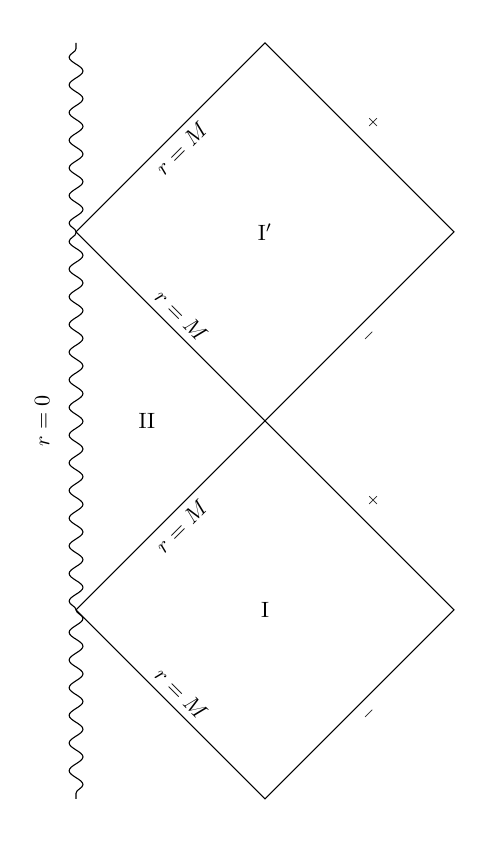
\begin{tikzpicture}[scale=0.6, every node/.style={scale=0.8}]
\node[above] (0) at (0.13,12) {};
\node[below] (1) at (0.13,-4) {};

\node (I) at (0,8) {I$^\prime$};
\node (II) at (0,0) {I};
\node (III) at (-2.5,4) {II};


\path % Four corners of left diamond
 (I) +(90:4) coordinate[label=90:] (IItop)
 +(-90:4) coordinate(IIbot)
 +(0:4) coordinate[label=360:] (IIright)
 +(180:4) coordinate[label=180:] (IIleft)
 ;
\draw (IIleft) --
 node[midway, below, sloped] {$r = M$}
 (IItop) --
 node[midway, above, sloped] {$\scri^+$}
 (IIright)
     node[midway, above, sloped] {}
           --
 node[midway, below, sloped] {$\scri^-$}
 (IIbot) --
 node[midway, above, sloped] {$r = M$}
 (IIleft) -- cycle;


\path % Four conners of the right diamond (no labels this time)
 (II) +(90:4) coordinate (Itop)
 +(-90:4) coordinate (Ibot)
 +(180:4) coordinate (Ileft)
 +(0:4) coordinate (Iright)
 ;
% No text this time in the next diagram
\draw (Ileft) --
 node[midway, below, sloped] {$r = M$}
 (Itop) --
 node[midway, above, sloped] {$\scri^+$}
 (Iright) --
 node[midway, below, sloped] {$\scri^-$}
 (Ibot) --
 node[midway, above, sloped] {$r = M$}
 node[midway, below, sloped] {}
 (Ileft) -- cycle;

%Squiggly lines
\draw[decorate,decoration=snake,draw=black] (Ileft) -- (IIleft)
 node[midway, above=0.3cm, sloped] {$r = 0$};


 % cut off top
 \draw[decorate,decoration=snake, draw=black] (-4,8) -- (-4,12)
 node[midway, below, sloped] {};
  % cut off bottom
 \draw[decorate,decoration=snake, draw=black] (-4,0) -- (-4,-4)
 node[midway, below, sloped] {};



%\draw[blue,dashed,bend right=25, thick] (Ileft) to (Iright);
%\draw[blue,dashed,bend right=-25, thick] (Ileft) to (Iright);
%\draw[blue,dashed,bend right=25, thick] (IIleft) to (IIright);
%\draw[blue,dashed,bend right=-25, thick] (IIleft) to (IIright);
%\draw[blue,dashed,bend right=25, thick] (Ileft) to (IIleft);
%\draw[blue,dashed,bend right=-25, thick] (Iright) to (IIright);
%\draw[->-,orange,bend right=-20, thick] (1) to (0);


\end{tikzpicture}
\caption[Penrose-Carter diagram for extremal Reissner-Nordstr\"om solution]{Segment of the Penrose-Carter diagram for extremal Reissner-Nordstr\"om solution. As with the non-extremal solution, this diagram can be extended above and below, infinitely.}
\label{fig:PenroseERN}
\end{figure}

\section{Calculating mass in general relativity}
\label{sec:gravitationalmass}
Our first experience of gravity in any formal way involves the notion of weight and with this, the concept of mass. It's then certainly a strange fact that when we consider a generic pseudo-Riemannian manifold $(M,g)$ in general relativity, there's not an obvious way to write down a sensible quantity for the mass. The diffeomorphism invariance within general relativity prevents us from assigning a total momentum four-vector, and as a result, we cannot the measure mass parameter \emph{\`a la} special relativity. If we wish to have a meaningful definition for a mass-like quantity in general relativity, we need some additional structure.

When we consider special relativity, we study some classical field with an associated energy-momentum tensor $T_{\mu \nu}$. Taking a slice of constant time to obtain a spacelike hypersurface $\Sigma$, with a unit normal $n^\mu$, the total energy associated with time translations generated by a Killing field $k^\mu$ is given by
	\begin{equation*}
		E = \int_{\Sigma} T_{\mu \nu} n^\mu k^\nu.
	\end{equation*}
As the energy-momentum tensor is conserved: $\partial_\mu T^{\mu \nu} = 0$, we understand $E$ to be independent of the choice of time slicing. This independence of the Cauchy surface $\Sigma$ is vital for the energy to be considered as a globally defined.
	
When we allow spacetime to be curved, the condition $\nabla_\mu T^{\mu \nu} = 0$ yields a local conservation law, but there is no invariant integral of $T^{\mu \nu}$ over an arbitrary region as $T^{\mu \nu}$ is not a differential form. As a result, we do not \emph{in general} have a global conservation law. An exception is when we have the additional structure of Killing vector field $k^\mu$ in the spacetime. We will elaborate on this further when we discuss the Komar mass. When a spacetime is asymptotically flat, the Arnott-Deser-Misner (ADM) construction can be used to define a total mass \cite{arnowitt1959}. In this formalism, the asymptotic limit is used to define a mass parameter in virtue of our understanding of a total momentum four vector in special relativity. In essence, asymptotically flat solutions can be considered isolated and the ADM mass measures a global energy density through calculating quantities in this limit. For spacetimes admitting Killing horizons with an asymptotically flat static region, the ADM formalism is equivalent to the Komar construction \cite{Ashtekar:1979cc}. As we will not be concerned with asymptotically flat spacetimes, we do not further comment on the ADM formalism.

After discussing the Komar mass, we then offer an alternative method to obtain a mass-like quantity quasi-locally. The Brown-York mass can be calculated in a spatially bounded region of spacetime providing that it is stationary. This method will be particularly important to us for the planar solutions we study in this thesis, where it found that the static regions of spacetime are of finite size.

When we interpret the law of black hole mechanics as a thermodynamic laws, we will see the mass parameter of black hole solutions plays the role of the internal energy of the system. As such, when we are looking to verify the first law of black hole mechanics it will be vital to compute a meaningful quantity associated to the mass parameter. Despite the usefulness of both the Komar mass and the Brown-York mass from the point of view of classifying the solutions within this thesis, we will see that they both suffer from an inability to be self-consistently normalised. Ultimately it is black hole thermodynamics itself that offers a way past this through the Euclidean action formalism. We expand on this in Section \ref{sec:eucldeanactionformalism}.

\subsection{Komar mass}
\label{sec:komarmass}
We begin our discussion of the Komar mass considering a spacetime $(M,g)$ which is stationary, \ie it admits a timelike Killing vector field $k^\mu$. We can understand the Komar mass as being the Noether charge associated to the symmetry associated with the Killing vector. Using the Killing vector, we can define a conserved current
\begin{equation*}
	J_\mu = - T_{\mu \nu} k^\nu, \qquad d \star J = 0,
\end{equation*}
where we use the language of forms, as it natural when considering Stoke's theorem. The total energy on a spacelike hypersurface $\Sigma$ is given by the integral
\begin{equation*}
	E_\Sigma = - \int_\Sigma \star J.
\end{equation*}
As the current is conserved, we can write the difference of two integrals over $\Sigma$ and $\Sigma^\prime$ bounding a region $N$ of spacetime and apply Stoke's theorem
\begin{equation*}
	E_{\Sigma^\prime} - E_\Sigma = - \int_{\partial N} \star J = - \int_{N} d \star J = 0.
\end{equation*}
From \eq{riekill}, we can associate covariant derivatives of the Killing vector field to the Riemann tensor. Contracting \eq{riekill}, we can relate the Killing vector to the Ricci tensor
\begin{equation*}
	\nabla^\nu \nabla_\nu k_\mu = - R_{\mu \nu} k^\nu,
\end{equation*}
and with Einstein's equations we have
\begin{equation*}
	- R_{\mu \nu} k^\nu =  8 \pi \left( T_{\mu \nu} - \half g_{\mu \nu} T \right) k^\nu.
\end{equation*}
We can see that the right-hand side of this term is conserved, and so we can write
\begin{equation*}
	d \star dk = 8 \pi \star \tilde{J}, \qquad \tilde{J}_\mu = 2 \left( T_{\mu \nu} - \half g_{\mu \nu} T \right) k^\nu,
\end{equation*}
where we have used Killing's equation to write
\begin{equation*}
	(\star d \star d k)_\mu = - \nabla^\nu \nabla_\mu k_\nu + \nabla^\nu \nabla_\nu k^\mu = 2 \nabla^\nu \nabla_\nu k^\mu = - 2 R_{\mu \nu} k^\nu.
\end{equation*}
We see that $\star \tilde{J}$ is exact and conserved, so we can write down the energy has an integral over the boundary of the hypersurface
\begin{equation}
\label{eq:komarenergy}
	E_\Sigma = - \int_\Sigma \star \tilde{J} = - \frac{1}{8\pi} \int_\Sigma d \star dk = - \frac{1}{8\pi} \int_{\partial \Sigma} \star dk .  
\end{equation}
We now have a covariant expression for a conserved charge generated by a timelike isometry, and we can interpret this as a measure of the total energy of spacetime. In its current form, this expression is dependent on the normalisation of the Killing vector field. In \cite{Komar:1958wp}, it is shown that this conserved charge can be considered as a mass for asymptotically flat spacetimes. In particular, it is shown that when the spacetime is asymptotically Schwarzschild at spatial infinity, the surface integral is evaluated in the asymptotic limit yields the $P^0$ term from the momentum four-vector in the asymptotic limit. This leads to the definition of the Komar mass

	\begin{defn}
	For an asymptotically flat, stationary spacetime $(M,g)$, the \emph{Komar mass} is the conserved charge associated with the timelike Killing vector field $k^\mu$
		\begin{equation}
		\label{eq:komarmass}
		    M_K = \lim_{r \rightarrow \infty} -\frac{1}{8 \pi} \int_{S^2} \star d k.
		\end{equation}	
		where the coordinate system is picked such that $r \rightarrow \infty$ is the asymptotically flat region. 
	\end{defn}

When a spacetime is equipped with a timelike Killing vector field, but is not asymptotically flat, a local-Komar like integral can be calculated without taking the limit to $r \rightarrow \infty$. We can still interpret this as a conserved quantity associated with the energy, but the overall normalisation is left unset. In Section \ref{sec:emconservedcharges} and Section \ref{sec:stumass}, we use this local form of the Komar integral to calculate a position dependent, mass-like parameter for our planar symmetric solutions.

\subsubsection*{Example: Reissner-Nordstr\"om solution}
As an example, let us calculate the Komar mass of the Reissner-Nordstr\"om solution. The Killing covector field in the static patch is given by
\begin{equation*}
	k = -f(r) dt, \qquad dk = \partial_r f(r) dt \wedge dr.
\end{equation*}
Computing the Hodge-star of $dk$ we find
\begin{equation*}
	(\star dk)_{\mu \nu} = \sqrt{-g}
 \; \varepsilon_{\mu \nu \rho \sigma} g^{\rho \tau} g^{\sigma \lambda} (dk)_{\tau \lambda} ,
 \end{equation*}
as the only non-zero term of $dk$ is the $t,r$ component, the only non-zero term of the Hodge dual is
\begin{equation*}
	(\star dk)_{\theta \phi} = - r^2 \sin \theta \cdot \partial_r f(r) = \left[- 2M + \frac{2e^2}{r} \right] \sin \theta.
\end{equation*}
Substituting this into \eq{komarmass}, we find that
\begin{equation*}
\begin{aligned}
M_K &= \lim_{r \rightarrow \infty} -\frac{1}{8 \pi} \left[- 2M + \frac{2e^2}{r} \right]  \int_{S^2} \sin \theta, \\
&= -\frac{4 \pi}{8\pi} \lim_{r \rightarrow \infty} \left( -2M + \Op(r^{-1}) \right), \\
&= M,
\end{aligned}
\end{equation*}
as expected.



\subsection{Brown-York mass}
\label{sec:brownyorkmass}

Much like we find that the local description for trapping horizons is more practical than the definition of event horizons, the Brown-York energy \cite{Brown:1992br} is useful in that we calculate it quasi-locally. The mass is derived via Hamilton-Jacobi analysis of the action functional for a gravitational system, in \cite{Brown:1992br}, it is shown that quasi-local energy is also the value of the Hamiltonian that generates unit magnitude proper-time translations. When the spacetime is also asymptotically flat, the Brown-York energy matches the mass derived from the ADM formalism, if the boundary of the calculation is taken to asymptotic infinity. In this section, we do not derive the form of the Brown-York energy, but instead write down the integral from \cite{Brown:1992br} and introduce the various components of the expression, such that we can calculate the Brown-York energy for our planar solutions throughout this thesis. 

The Brown-York quasi-local energy is found from\footnote{Alternative treatments of the quasi-local energy include the lapse function $N$ into the expression \cite{Katz_1988}, which has an effect on non-asymptotically flat spacetimes. In this section we follow the work of Brown and York and do not include the lapse function.}

\begin{equation}
\label{eq:BYmass}
E_{BY} = -\frac{1}{8 \pi} \int_{B} \sqrt{\sigma} (\mathtt{k} - \mathtt{k}_0),
\end{equation}
where we use the notation of $\mathtt{k}$ as the extrinsic curvature of the codimension-two manifold $B$ embedded within $M$, where $\sigma$ is the metric of $B$ and $\mathtt{k}_0$ is a background contribution. In the following discussion, we will better introduce all these pieces to the reader.

In this formalism, we consider a physical spacetime $(M,g)$, which is topologically a hypersurface $\Sigma$, foliated over a real line interval: $M = \Real \times \Sigma$. We denote boundary of $\Sigma$ as $B$, a codimension-two manifold in $M$. Taking the product of $B$ with the timelike worldlines orthogonal to $\Sigma$ produces the codimension-one hypersurface ${}^3B$, a component of the three-boundary of $M$. The full boundary of $M$ includes the end points of timelike worldlines.

\begin{figure}[h!]
\centering
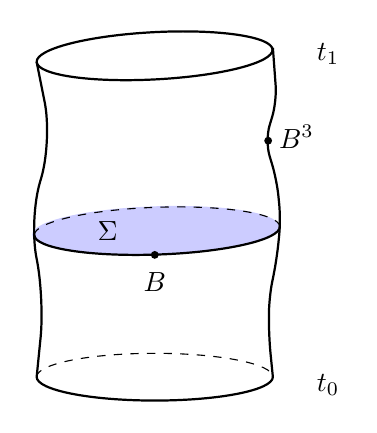
\begin{tikzpicture}
	\draw[thick, rotate around={3:(-1.5,2)}] (-1.5,2) arc (180:360:1.5cm and 0.3cm);
	\draw[thick, rotate around={3:(-1.5,2)}] (-1.5,2) arc (180:0:1.5cm and 0.3cm);
	
	\draw[thick] (-1.5,-2) arc (180:360:1.5cm and 0.3cm);
	\draw[dashed] (-1.5,-2) arc (180:0:1.5cm and 0.3cm);
	
	\begin{scope}[shift={(1.51,0.06)}]
	\draw[color=blue!20!white, fill=blue!20!white, rotate around={2:(-1.5,-0.2)}] (-1.5,-0.2) ellipse (1.56cm and 0.3cm);
	\end{scope}
	
	\begin{scope}[shift={(-0.03,0)}]
	\draw[thick, rotate around={2:(-1.5,-0.2)}] (-1.5,-0.2) arc (180:360:1.56cm and 0.3cm);
	\draw[dashed, rotate around={2:(-1.5,-0.2)}] (-1.5,-0.2) arc (180:0:1.56cm and 0.3cm);
	\end{scope}
	
	\draw[rounded corners=5mm, thick](-1.5, 2) -- (-1.3, 1) -- (-1.6, 0) -- (-1.4, -1) -- (-1.5, -2);
	\draw[rounded corners=2mm, thick](1.5, 2.18) -- (1.55, 1.5) -- (1.4, 1) -- (1.55, 0.5) -- (1.6, 0) -- (1.55, -0.5) -- (1.45, -1) -- (1.45, -1.5) -- (1.5, -2);
	
	\node (0) at (-0.6,-0.15)   {$\Sigma$};
	\node at (0,-0.45) [circle,fill,inner sep=1pt]{};
	\node (0) at (0,-0.8) {$B$};
	
	\node at (1.44,1) [circle,fill,inner sep=1pt]{};
	\node (0) at (1.8,1.05) {$B^3$};
	
	\node (0) at (2.2, 2.1) {$t_1$};
	\node (0) at (2.2, -2.1) {$t_0$};
\end{tikzpicture}
\label{fig:}
\caption[Illustration of manifold structure for Brown-York quasi-local energy]{The manifold $M$, which topologically $\Real \times \Sigma$. Taking a surface of constant $t$, we obtain the codimension-one hypersurface $\Sigma$. The boundary of $\Sigma$ is the codimension-two hypersurface $B$. Taking the product $\Real \times B$, we obtain the codimension-one hypersurface $B^3$.}
\end{figure}

To calculate \eq{BYmass}, we will need the geometric data of $B$ in terms of the known data of $(M,g)$. We take a future pointing unit vector $u^\mu$, normal to the foliation $\Sigma$. A tensor $T$ is said to be spatial when $T\cdot u=0$. The metric $g_{\mu \nu}$ induces a metric on $\Sigma$, which, when regarded as a tensor $h_{\mu \nu}$ on $M$, is a spatial tensor. The induced covariant derivative $\D_\mu$ for spatial tensors is found through projection $\D_\mu = h^\nu_\mu \nabla_\nu$. The extrinsic curvature of $\Sigma$ as an embedded submanifold of $M$ is denoted $K_{\mu \nu}$. We use the notation $h_{ij}, \; K_{ij}$, where $i,j$ run from one to the dimension of $\Sigma$, when regarding the metric and extrinsic curvature of $\Sigma$ as tensors on $\Sigma$. 

The ADM decomposition \cite{arnowitt1959} of the metric is given by
\begin{equation}
\label{eq:ADM}
    ds^2 = -N^2 dt^2 + h_{ij} (dx^i + V^i dt)(dx^j + V^j dt),
\end{equation}
for a lapse function $N$ and shift vector $V^i$.

We proceed in the same way with the three-boundary ${}^3B$ by considering the outward pointing unit vector $n^\mu$, normal to ${}^3B$. The metric induced by $g_{\mu \nu}$ is denoted $\gamma_{mn}$ when regarded as a tensor on ${}^3B$ and $\gamma_{\mu \nu}$ when regarded as a horizontal tensor on $M$, \textit{i.e.} as a tensor $T$ on $M$ satisfying $n\cdot T = 0$. 

The boundary $B$, which is the intersection of $\Sigma$ and ${}^3B$, has a metric $\sigma_{\mu\nu}$ which can be induced from either of the codimension-one manifolds or the spacetime itself. The extrinsic curvature $\mathtt{k}_{\mu\nu}$ of $B$ – the vital part needed to calculate \eq{BYmass} – is computed using the embedding of $B$ in $\Sigma$:
\begin{equation}
\begin{aligned}
\label{eq:extexplicit}
\mathtt{k}_{\mu \nu} &= \sigma^\alpha_\mu \D_\alpha n_\nu, \\
&= \gamma^\alpha_\mu h^\beta_\nu h^\rho_\alpha \nabla_\rho n_\beta   . 
\end{aligned}
\end{equation}
We will also need the trace $\mathtt{k} = \sigma^{\mu\nu} \mathtt{k}_{\mu \nu}$ in our later calculations.

The last piece of \eq{BYmass} to comment on is the background normalisation term $\mathtt{k}_0$. When working with the action, there is an inherent ambiguity on the boundary, which in its most general form is built from data on $\gamma_{mn}$. In \cite{Brown:1992br}, the subtraction term is set by ensuring the energy density depends only on canonical variables. The quasi-local energy is shown to obey additivity, and so we can understand $\mathtt{k}_0$ as a term removing the contribution from flat Minkowski space, which intuitively we would expect to have a zero energy density. For the derivation, and an explanation of how the action functional relates to the extrinsic curvature of the boundary $B$, we refer to \cite{Brown:1992br}.

It is then shown that calculating the energy when boundary is taken in the asymptotic limit, the quasi-local energy is the same as the ADM mass for asymptotically flat spacetimes. Alternatively, taking the Newtonian limit of the quasi-local energy for a spherical distribution of mass of radius $R$ and mass $M$, it is shown that the quasi-local energy takes the form
\begin{equation*} 
E_{BY} \simeq M + \frac{2M}{R}.
\end{equation*} 
We interpret these as the contributions from the matter energy density and the Newtonian gravitational potential energy, and so we can see $E$ as a natural description for the total energy of the system within this boundary.

\subsubsection*{Example: Reissner-Nordstr\"om solution}

It is instructive to perform the calculation for the Brown-York quasi-local energy for a solution we already have experience with, before applying it to the novel solutions of this thesis. In this section, we calculate the quasi-local energy of the Reissner-Nordstr\"om solution, and show that by taking the asymptotic limit we recover the Komar mass calculated in Section \ref{sec:komarmass}.

We will need to calculate the trace of the extrinsic curvature $\mathtt{k}$ for both the Reissner-Nordstr\"om metric and $\mathtt{k}_0$ for the Minkowski metric. In the following we will use the metric:
\begin{equation*}
	ds^2 = -f(r) dt^2 + f(r)^{-1} dr^2 + d\Omega^2, \qquad f(r) = \left(1 - \frac{2M}{r} + \frac{e^2}{r^2} \right),
\end{equation*}
but keep the function $f(r)$ general as much as we can, which will help for calculations later. We also realise we can get results for the Minkowski solution by allowing $f(r) = 1$. Comparing the Reissner-Nordstr\"om metric with the ADM decomposition \eq{ADM} we can identify the lapse and shift functions
\begin{equation*}
N^2 = f(r), \qquad V^i = 0.
\end{equation*}
The outward point unit normal we consider is $n^{\mu} = \left(0,\sqrt{f(r)},0,0 \right)$, such that $n^2 = 1$. 

To calculate the Brown-York energy, we need to calculate the extrinsic curvature of the manifold $B$ embedded into the spacetime $M$ with \eq{extexplicit}. Computing this and taking the trace, we find
\begin{equation*}
	\mathtt{k} = \sigma^{\mu \nu} \mathtt{k}_{\mu \nu} = \frac{2 \sqrt{f(r)}}{r}, \qquad \mathtt{k}_0 = \frac{2}{r}.
\end{equation*}
For Reissner-Nordst\"om, the boundary $B$, with metric $\sigma_{\alpha \beta}$ is the two-sphere with radius $r$ set for the boundary location.

We now have all the necessary pieces to calculate the Brown-York energy
\begin{equation*}
	\begin{aligned}
		E_{BY} &=  -\frac{1}{8 \pi} \int_{B} \sqrt{\sigma} (\mathtt{k} - \mathtt{k}_0) ,\\
		&=  -\frac{1}{8 \pi} \int_{B} r^2 \sin \theta \left( \frac{2 \sqrt{f(r)}}{r} - \frac{2}{r} \right) ,\\
		&=  r \left( 1 - \sqrt{f(r)}  \right).
	\end{aligned}
\end{equation*}
We see that in the limit of setting the boundary for $r \rightarrow \infty$, the quasi-local energy takes the form
\begin{equation*}
	M_{BY} := \lim_{r \rightarrow \infty} E_{BY} \approx \left( M + \frac{M^2 - e^2}{2r} + \Op(r^{-2})  \right),
\end{equation*}
and so the constant contribution is the mass parameter of the solution $M$, which is precisely the ADM mass for asymptotically flat solutions. We see that the energy contributions from the $\Op(r^{-1})$ order terms can be understood as the gravitational binding energy, and the electrostatic binding energy. We note here that if we were to include the lapse function to the quasi-local energy following \cite{Katz_1988}, both of these sub-leading contributions would be positive.


\section{Black hole thermodynamics}
\label{sec:bhthermo}

In this section, we introduce the laws of black hole mechanics, a set of geometric relationships built from the properties of black hole solutions. A truly remarkable feature of black holes is uncovered through these rules; by interpreting the surface gravity and the area of the black hole as the temperature and entropy of some thermodynamic system, the laws of black hole mechanics can be understood as the laws of thermodynamics. This similarity has a deeper physical connection and by considering black holes semi-classically, the thermodynamic interpretation of a black hole can be formalised. The work started with the concept of the entropy of a black hole being proportional to its area, rather than its volume. In 1972, Bekenstein conjectured \cite{Bekenstein:1973ur} that the entropy of a black hole would be proportional to the area of the black hole divided by the Planck length squared. Soon after, Hawking was able to set the constant of proportionality and proved Bekenstein's conjecture by considering a quantum field theory in a curved background \cite{Hawking:1974sw}. Looking at quantum fluctuations near the event horizon, Hawking proved that stationary black holes emitted thermal radiation as a blackbody. We will discuss the temperature of black holes and the seeming contradiction of a black hole emitting heat in more detail in Section \ref{sec:bhtemperature}. 

In this section, we outline the four rules of black hole mechanics and remark on their similarity to the laws of thermodynamics. In Appendix \ref{app:thermo}, we expand on the thermodynamic laws themselves and elaborate on a few extra details that will be useful when we consider the Euclidean action formalism in Section \ref{sec:eucldeanactionformalism}.

\subsection{Laws of black hole mechanics}

\paragraph{Zeroth law of black hole mechanics} 

The zeroth law is the statement that the surface gravity is constant across a future event horizon. As we have most of the pieces already discussed to prove this, we offer a formal proof of this law. 

\begin{thm}[Zeroth Law of Black Hole Mechanics]
	The surface gravity $\kappa$ is constant on a future event horizon $\Ham^+$, for a stationary spacetime obeying the dominant energy condition \cite{Bardeen:1973gs}.  
\end{thm}

\begin{proof}

In this proof, we use Hawking's theorem that an event horizon $\Ham^+$ is a Killing horizon with respect to a Killing vector field $\xi^\mu$ \cite{Hawking:1973uf}, and so we will show that the surface gravity $\kappa$ is constant on a Killing horizon $\N$. This roughly follows the proof given in \cite{Bardeen:1973gs}.

Raychaudhuri's equation \cite{Poisson:2009pwt} relates the expansion, shear and twist of a null congruence, with generators $U^\mu$ to the Ricci tensor by
\begin{equation*}
	\diff{\theta}{\lambda} = - \half \theta^2 - \hat{\sigma}^{\mu \nu} \hat{\sigma}_{\mu \nu} + \hat{\omega}^{\mu \nu} \hat{\omega}_{\mu \nu} - R_{\mu \nu} U^{\mu} U^{\nu}.
\end{equation*}
On a Killing horizon we have seen that, $\theta = \hat{\sigma} = \hat{\omega} = 0$ and Raychaudhuri’s equation simplifies to
\begin{equation*}
	0 = R_{\mu \nu} \xi^\mu \xi^\nu \; \big|_{\N} = 8\pi T_{\mu \nu} \xi^\mu \xi^\nu,
\end{equation*}
where we have used Einstein's equation and $\xi^2 |_{\N} = 0$ in the last step. From this, we see that on the Killing horizon, we can write down a current $J_\mu = - T_{\mu \nu} \xi^\nu$. The dominant energy condition states that $- T^{\mu}_{\nu} X^\nu$ is future-directed for all future-directed vector fields $X^\mu$. As the Killing vector field is future-directed, so is $J_\mu$ and hence the current must be parallel to the Killing vector field.

We can then antisymmetrise and with \eq{riekill} and write down
\begin{equation*}
	0 = \xi_{[\mu} J_{\nu]} =- \frac{1}{8\pi} \xi_{[\mu} R_{\mu] \rho} \xi^\rho  = \frac{1}{8 \pi} \xi_{[\mu} \partial_{\nu ]} \kappa,
\end{equation*}
and so $\partial_\mu \kappa$ must be proportional to $\xi_\mu$ and hence $X^\mu \partial_\mu \kappa = 0$ for a vector field $X^\mu$ tangent to $\N$. We then understand $\kappa$ is constant on the Killing horizon. 
\end{proof}

Looking at this result, with the not-so-subtle naming of it as the \emph{zeroth law}, we can think about the zeroth-law of thermodynamics, which states that for a body in equilibrium, the temperature is constant.

\paragraph{First Law of Black Hole Mechanics}

The no hair theorem of Wheeler \cite{Misner:1974qy, Israel:1967wq} states that stationary black hole solutions are completely encoded by their mass $M$, electromagnetic charges $\mathcal{Q}_i$ and their angular momentum $J$. By varying these parameters, we find a differential relationship
\begin{equation}
\label{eq:firstlaw}
	\frac{\kappa}{8 \pi} dA  = dM - \Omega_H J - \mu d\mathcal{Q},
\end{equation}
where the $\Omega_H$ is the angular velocity of a rotating black hole solution and $\mu$ is the chemical potential, which can be computed from the asymptotic value of the time component of the gauge-fixed vector potential \cite{Hartnoll:2009sz}. For all the solutions within this thesis, $\Omega_H = J = 0$, but we include it here for generality; the canonical example of spinning black holes is the Kerr solution \cite{Kerr:1963ud}. We can understand the first law of black hole mechanics as the statement of energy conservation for a black hole solution. It has been proved for stationary black hole solutions by Sudasky and Wald \cite{Sudarsky:1992ty}. In this thesis, we will show that the first law is also satisfied for a class of Killing horizons where the external, asymptotic region of the spacetime is time-dependent. Hartle and Hawking \cite{Hawking:1972hy} proved an alternative version of the first law by perturbing a black hole solution by adding some small mass $\delta M$ to a black hole and letting the spacetime settle back to a stationary solution, and an alternative proof is found in \cite{Bardeen:1973gs} by Bardeen, Carter and Hawking.

As an example, we can verify the first law for the Reissner-Nordstr\"om solution, where in Section \ref{sec:rnsol} we found that $\mathcal{Q} = Q$, $r_\pm = M \pm \sqrt{M^2 - Q^2}$ and for the Killing horizon at $r = r_+$, the surface gravity is $\kappa = (r_+ - r_-) / r_+^2$:
\begin{equation*}
\begin{aligned}
	\frac{\kappa}{8 \pi} d A &= \frac{\kappa}{2} d (r_+^2) = \frac{\sqrt{M^2 - Q^2}}{r_+} d \left(M + \sqrt{M^2 - Q^2} \right)  \\
	&= \frac{\sqrt{M^2 - Q^2}}{r_+} \left[dM + \frac{1}{2\sqrt{M^2 - Q^2}} \left( 2MdM - 2QdQ \right) \right] \\
	&= \left(\frac{\sqrt{M^2 - Q^2}}{r_+} + \frac{M}{r_+} \right) dM - \frac{Q dQ}{r_+} \\
	&= dM - \mu d\mathcal{Q},
\end{aligned}
\end{equation*}
where we have used Equation \eq{rnchempot} for the chemical potential $\mu$.

Understanding the mass as encoding the total energy of the black hole, this relationship is tantalisingly close to the first law of thermodynamics
\begin{equation*}
	dE = T dS + \mu_i d\mathcal{Q}_i - PdV,
\end{equation*}
where the $\mu_i d\mathcal{Q}_i$ terms encode the work terms associated to the system, and $PdV$ is the term associated to the pressure / volume of the closed system. For us to relate these two differential relationships, we must associate $T dS$ with the geometric terms $\frac{1}{8\pi} \kappa dA$. 

\paragraph{Second Law of Black Hole Mechanics}

The second law of black hole mechanics is Hawking's area law \cite{Hawking:1971vc}. Informally, this law states that if one assumes both the cosmic censorship conjecture and the null energy condition, the area $A$ of an event horizon $\Ham$ does not decrease with time
\begin{equation*}
	\delta A \geq 0.
\end{equation*}
We have not formally defined either of these two assumptions in this thesis as they are not vital to the work in the main body. As a sketch, the (weak) cosmic censorship is the statement that all singularities in the spacetime are hidden behind a horizon and the null energy condition states that for a null vector field $X^\mu$ we have the inequality $T_{\mu \nu} X^\mu X^\nu \geq 0$. 

The first law seemed to suggest that the area and entropy were proportional. We can follow this into the second law and realise Hawking's area theorem is then the statement that for a physical process, the entropy of a black hole would be always increasing. This relationship is perhaps the most interesting. Hawking's area theorem is a rigorous geometric statement from the geometry of spacetime, but the second law of thermodynamics is a classical result which is believed to hold for systems with a large number of particles. 

There is a slight modification to this story when we take seriously the notion of thermal radiation from a black hole with temperature proportional to $\kappa$. Over time, a black hole will eventually evaporate and while doing so, lose entropy through the thermal radiation. Taking this into account, the second law is generalised such that combination of the black hole's entropy together with the entropy encoded into the radiation is non-decreasing: $\delta(S_{BH} + S_{T}) \geq 0 $\cite{BekensteinGeneralised}. We will not comment further on this.

\paragraph{Third Law of Black Hole Mechanics}

The third law is less well defined, from both the thermodynamic and black hole perspectives, and in fact comes in two versions: the strong and the weak third law. Unlike the last three, we will state the third law as a thermodynamic law and then refer to the geometric formulation for the third law(s) as they currently stand.

The weak version of the third law states that the temperature of a system cannot be reduced to zero in a finite number of steps, in which the entropy is at the minimum value. A stronger version put forward by Planck \cite{landau2013statistical} states that the entropy vanishes when the system is brought to zero temperature.

From a geometric perspective, Israel put forward a formulation \cite{Israelthird} that it is impossible to reduce the surface gravity to zero in a finite number of steps. However, there is no form of proof for the third law, in fact, we already have a counter example with the extremal Reissner-Nordstr\"om solution. In this solution, the surface gravity of the solution vanishes, and yet there is still a black hole with a finite size! The third law may have ambiguities, but it's still an active area of research in black hole physics \cite{ Page:1976ki, Wald:1997qp, Hartnoll:2007ih, DHoker:2009ixq}. In \cite{Barisch:2011ui, Cardoso:2015wcf, Dempster:2015, Dempster:2016} a class of black hole solutions dubbed \emph{Nernst branes} were found in $\N = 2$ gauged supergravity with the special property that they obeyed the strong version of the third law. These solutions were the starting-off point for the class of solutions found in \cite{Gutowski:2019iyo}, the research of which is one of the main results of this thesis. Further discussion of Nernst branes is delayed until Chapter \ref{ch:planarstu}. We can summarise these results into Table \ref{table:laws} \cite{Wald:106274}.

\begin{table}[h!]
\centering
\def\arraystretch{1.3}
\begin{tabular}{|p{1.5cm}|p{5.5cm}|p{5.5cm}|}
\hline
{Law}    & {Black Hole Mechanics}                                             & {Thermodynamics}                                                \\ \hline \hline
Zeroth & $\kappa$ is constant over the horizon of a stationary black hole & $T$ is constant for a body in equilibrium                     \\ \hline 
First  & $dM = \frac{1}{8\pi} \kappa dA + \mu d\mathcal{Q} + \Omega_H dJ$ & $dE = T dS + \mu_i dC_i - P dV$   \\ \hline
Second & $\delta A \geq 0$  for physical processes                                               & $\delta S \geq 0$ for physical processes                                            \\ \hline
Third  & The surface area is minimised for extremal black holes           & The entropy is minimised at absolute zero \\ \hline
\end{tabular}
\caption[Comparison of the laws of black hole mechanics and thermodynamics]{A summary of the laws of black hole mechanics and a comparison of their form to the laws of thermodynamics.}
\label{table:laws}
\end{table}

\subsection{Temperature of horizons}
\label{sec:bhtemperature}
Realising the laws of black hole mechanics as thermodynamic relations leads to a new interpretation for geometric parameters associated to the black hole solution. From the zeroth and first law, we are led to related the surface gravity to temperature, and from the first and the second laws, we relate the area of a black hole as a measure of its entropy. We can formalise this in the following way
\begin{equation*}
	T = \alpha \kappa, \qquad S = \frac{A}{8 \pi \alpha},
\end{equation*}
where we allow some constant $\alpha$, which we cannot set from the mechanical laws alone. This leads to a strange contradiction. By definition, a black hole is a region of spacetime from which nothing can be emitted, but the interpretation of a black hole as a thermodynamic object leads us to interpret it as some blackbody radiating with a temperature $T_H$. 

It was Hawking in 1974 \cite{Hawking:1974sw} that was able to reconcile this by studying the black hole semi-classically. By considering matter quantum mechanically, Hawking showed that a black hole radiates as a blackbody with a temperature
\begin{equation}
\label{eq:hawkingtemp}
	T_H = \frac{\kappa \hbar}{2\pi k_B c},
\end{equation}
where we have re-introduced all physical constants briefly. There is something beautiful in the collision of so many areas of physics in this one equation. Hawking's derivation sets the value of the constant $\alpha$, and with this validated Bekenstein's conjecture that the entropy of a black hole should be proportional to its area divided by the Planck length squared \cite{Bekenstein:1973ur}
\begin{equation}
\label{eq:bhentropy}
	S_{BH} = \frac{k_B A c^3}{4 G \hbar} = \frac{k_B A}{4 \ell_P^2}.
\end{equation}
For the remainder of our discussion, we return back to our conventions of suppressing physical constants such that
\begin{equation*}
	T = \frac{\kappa}{2\pi}, \qquad S = \frac{A}{4}.
\end{equation*}

Hawking's work means that given a Killing horizon, one can calculate the surface gravity of the horizon and hence the temperature. However, given a Killing horizon $\N$, with a Killing vector field $\xi$, and surface gravity $\kappa$, $\N$ is also a Killing horizon of $\alpha \xi$ with surface gravity $\alpha^2 \kappa$ for any constant $\alpha$. This means that the surface gravity is not a unique property of $\N$ and depends on the normalisation of the Killing vector. As the norm of the Killing vector vanishes on the hypersurface, there is no way to normalise $\xi$ on $\N$ in a natural way.

When a spacetime is stationary and asymptotically flat, there is a natural normalisation that allows us to set the time-translation Killing vector $k$ with that of Minkowski space:
\begin{equation*}
	\lim_{r \rightarrow \infty} k^2 = -1.
\end{equation*}   
However, when a spacetime does not admit an asymptotically flat spacetime, the surface gravity, and hence the temperature, must be set in another setting.

An alternative calculation for the Hawking temperature comes from studying the Euclidean section of a black hole solution by Wick-rotating the time coordinate $t \rightarrow -i \tau$. In the next section, we show that the Wick-rotation goes beyond just a calculation for the temperature but all the way to a thermodynamic partition function.

After Wick-rotation, the coordinate $\tau$ must be periodically identified $\tau \simeq \tau + \beta$, where $\beta = T_H^{-1}$ is the inverse temperature. This identification is imposed to ensure the absence of a conical singularity at the origin of the Euclidean manifold. 

Taking a black hole solution with a line element of the form
\begin{equation*}
	ds^2 = - f(r) dt^2 + \frac{dr^2}{f(r)} + r^2 d\vec{X}^2, 
\end{equation*}
where $d\vec{X}^2$ is a generic line element for a two-dimensional space. Conventionally this would be the two-sphere $S^2$ and later it will be the plane $\Real^2$ for our planar symmetric solutions. The function $f(r)$ has a zero for $f(r_h) = 0$, with a non-zero derivative. We can write down the approximation for line element near the Killing horizon at $r = r_h$ by Taylor-expanding
\begin{equation*}
	ds^2 = - \partial_r f(r_h) (r - r_h) dt^2 + \frac{dr^2}{\partial_r f(r_h) (r - r_h)} + r_h^2 d\vec{X}^2.
\end{equation*}
Wick-rotating $t \rightarrow -i \tau$, we can write down the line element as 
\begin{equation*}
	ds^2 = \rho^2 d\theta^2  + d\rho^2 + r_h^2 d\vec{X}^2,
\end{equation*}
where we have made the additional coordinate transformation
\begin{equation*}
	\rho^2 = \frac{4(r - r_h)}{\partial_r f(r_h)}, \qquad \theta = \half \partial_r f(r_h) \tau.
\end{equation*}
We see that the conical singularity from the Wick-rotation is avoided as long as we make the identification
 \begin{equation*}
 	\theta \simeq \theta + 2 \pi, \quad \Rightarrow \quad \tau \simeq \tau + \frac{4 \pi}{\partial_r f(r_h)},
 \end{equation*}
 and so we find that the temperature of the solution found from Wick-rotating is given by
 \begin{equation*}
 	T_H = \frac{\partial_r f(r_h)}{4 \pi}.
 \end{equation*}
 As a consistency check for this calculation, we can calculate the surface gravity using the Killing vector filed $k^\mu = \partial_t$ and Equation \eq{surfacegravity} and we find
 \begin{equation*}
 	\kappa = \half \partial_r f(r_h),
 \end{equation*}
 where in order to evaluate the result on the horizon at $r = r_h$, it is necessary to perform an Eddington-Finkelstein transformation on the line element first. With this expression for $\kappa$, we can see that the temperature calculated from the Wick-rotation matches \eq{hawkingtemp}. We can notice that $\theta = \kappa \tau$, but when studying the line element, the surface gravity enters the line element quadratically and so this procedure doesn't actually determine whether $T_H$ is positive or negative. 

The ambiguity in the scaling and sign of the temperature of a black hole solution ultimately requires the full computation of Hawking temperature using curved spacetime quantum field \cite{Hawking:1974sw}, or the tunnelling effect for a quantum particle \cite{Parikh:1999mf}. For stationary, asymptotically flat spacetimes, Hawking's work holds and computation of the temperature can be done with either of the above methods. However, for the solutions we consider within this thesis, we will need to extend our work suitably to understand the Killing horizons of our solutions. 

Deriving the temperature of a Killing horizon by considering the semi-classical emission of black body radiation is a complicated set of calculations, especially as it seems that all we want is to set the sign of the temperature for non-standard black hole solutions. However, there is a known relation for the sign of the temperature for the four variants of trapped horizons defined in Section \ref{sec:horizonclassify}. In particular, we will be concerned with regions of spacetime which depended on a timelike coordinate $t$. For these solutions, the absence of a timelike Killing vector field inhibits the canonical computation of the surface gravity. However, by following the work of \cite{Hayward:1997jp}, the surface gravity can be computed using the Kodama vector \cite{Kodama:1980}. With a valid expression for the surface gravity, following the work of \cite{Binetruy:2014ela, Helou:2015zma}, we can show that once the category of trapping horizon is identified the sign of the temperature is fixed.

The Kodama-Hayward surface gravity can be computed when the metric has the structure
\begin{equation*}
    ds^2 = \gamma_{ij}(x) dx^i dx^j + C^2(x) d\vec{X}^2 \;,\quad i=0,1,
\end{equation*}
where $\gamma_{ij}$ and $C$ only depend on the coordinates $(x^0,x^1) = (t,r)$. For spherically symmetric spacetimes, $d\vec{X}^2 = d\Omega_2$ is the standard metric on the two-sphere. In our later calculations, we will allow planar symmetry and hence $d\vec{X}^2$ is the standard metric on $\mathbb{R}^2$. The surface gravity in the Kodama-Hayward formalism is
\begin{equation*}
    \kappa = \frac{1}{2 \sqrt{-\gamma}} \partial_i \left(\sqrt{-\gamma} \gamma^{ij} \partial_i C 
    \right) = \frac{1}{2}
    \Delta_\gamma C \;.
\end{equation*}
For later reference, we compute the Kodama-Hayward surface gravity for line elements
of the form 
\begin{equation*}
    ds^2 = - \frac{dt^2}{f(t)} + f(t) dr^2 + t^2 d\vec{X}^2,
\end{equation*}
which include the dynamic patches of the solutions considered within this thesis. Performing the computation, we find that the surface gravity is given by
\begin{equation}
\label{eq:THK}
\kappa = -\frac{1}{2} \partial_t f(t_h), \qquad f(t_h) = 0.
\end{equation}

Following \cite{Binetruy:2014ela, Helou:2015zma}, trapping horizons and their Kodama-Hayward surface gravity subdivide into four cases as the sign of the surface gravity is proportional to
\begin{equation*}
	\kappa \propto -  \La_{\ell_\mp} \theta_\pm.
\end{equation*}
Thus outer horizons have positive surface gravity, while inner horizons have negative surface gravity. By computing the Hawking temperature of a trapping horizon using the Parikh-Wilczek tunnelling method,   \cite{Parikh:1999mf, Binetruy:2014ela, Helou:2015zma}, we find an additional sign between the Hawking temperature and the surface gravity for trapping horizons with $T_H \propto \pm \kappa$, with the $(+)$ sign for future horizons and the $(-)$ sign for past horizons. We can summarise these signs
\begin{enumerate}[(i)]
	\item \emph{Future outer horizons}
	\begin{equation*}
		\theta_+ = 0, \;\; \theta_- < 0, \;\; \La_{\ell_-} \theta_+ < 0, \qquad  \qquad\kappa > 0, \;\; T_H > 0.
	\end{equation*}
	\item \emph{Past outer horizons}
	\begin{equation*}
		\theta_- = 0, \;\; \theta_+ < 0, \;\; \La_{\ell_+} \theta_-  < 0, \qquad \qquad \kappa >  0, \;\; T_H < 0.
	\end{equation*}
		\item \emph{Future inner horizons}
	\begin{equation*}
		\theta_+ = 0, \;\; \theta_- < 0, \;\; \La_{\ell_-} \theta_+ > 0, \qquad \qquad \kappa <  0, \;\; T_H < 0.
	\end{equation*}
	\item \emph{Past inner horizons}
	\begin{equation*}
		\theta_- = 0, \;\; \theta_+ < 0, \;\; \La_{\ell_+} \theta_-  > 0, \qquad \qquad \kappa <  0, \;\; T_H > 0.
	\end{equation*}
\end{enumerate}
The net effect is that future outer horizons (black holes), and past inner horizons (expanding cosmologies) have positive temperature, while future inner horizons (contracting cosmologies) and past outer horizons (white holes) have negative temperature. 

Negative temperature has been argued to indicate the absence of Hawking radiation, since future inner and past outer horizons cannot separate virtual particle pairs created by vacuum fluctuations, thus not enabling the Hawking effect \cite{Binetruy:2014ela, Helou:2015zma}. However, in thermodynamics, the inverse temperature is related to the entropy $S$ and internal energy $E$ by
\begin{equation*}
    \beta = \pardev{S}{E}.
\end{equation*} 
Therefore, negative temperature can occur if one drops the usual assumption that the entropy increases monotonically with the energy. A toy model for negative temperature is provided by a system with finite maximum energy \cite{Ramsey:1956}. Taking a system with two energy eigenstates $E_1< E_2$ as the simplest example, this will be in a maximally ordered state $(S=0)$ if all particles are either in the lower or in the higher state, while a maximally disordered state is realised when half of the particles are in either state. Upon heating up such a system, entropy and temperature first increase, with the temperature reaching $+\infty$  when entropy becomes maximal. Upon further heating, the entropy decreases and the temperature jumps at the turning point from $+\infty$ to $-\infty$. After this point, it increases, approaching $0$ from below when reaching a situation where all particles are in the higher state. Thus negative temperatures are `higher' than positive temperatures and correspond to `population inversion.' We will see later that some of the horizons we are interested in have negative surface gravity and negative temperature, and that this is necessary in order for the first law to take its standard form when using our triple Wick-rotated Euclidean formalism.

\section{Euclidean action formalism}
\label{sec:eucldeanactionformalism}
One of the main results of this thesis is the verification of the first law of Killing horizon mechanics for a class of planar symmetric, cosmological solutions of Einstein-Maxwell and $\N = 2$ supergravity theories. As mentioned, these solutions are neither asymptotically flat, nor stationary in the exterior regions of the spacetime, complicating our ability to find a meaningful mass parameter from which we could verify the first law. Both the Komar mass and Brown-York mass can be used to find local mass-like parameters within the finite, static region of our solutions, but both of these methods have a freedom in their normalisation, and so the first law -- a differential relationship -- cannot be studied without imposing an additional condition.

The Euclidean action formalism \cite{Gibbons:1976ue, Gibbons:1977mu} is a method to study the thermodynamics of black holes through the formal identification of the gravitational partition function and the thermodynamic partition function. This procedure leads to the computation of a thermodynamic potential by its relation to the Euclidean action of the gravitational theory. We can calculate various thermodynamic parameters such as the mass, charge, entropy and temperature from derivatives of the thermodynamic potential. More details are given in Appendix \ref{app:thermo}. In our solutions, we find the natural thermodynamic potential related to the Euclidean action for theories with electromagnetic charges is the grand potential $\Omega(\beta, \mu)$ and via a Legendre transformation, we compute the free energy $F(\beta, \mathcal{Q})$.

For planar symmetric solutions, a normalisation ambiguity remains in the Euclidean action formalism, but we can now set it with the additional condition that the charge calculated from the grand potential matches the charge calculated from Gauss' law. This sets an overall numerical factor for the Euclidean action, and hence the remaining thermodynamic variables. For asymptotically flat spacetimes, this normalisation is unnecessary as we have the Minkowski solution at infinity to normalise as a background contribution. With the normalisation set, we show the thermodynamic entropy matches the Bekenstein area law, and we derive a mass parameter. This mass parameter can be varied and the first law verified.

In this section, we introduce the Euclidean action formalism using the Reissner-Nordstr\"om solution as an example. We work through a computation of the Euclidean action, together with the background terms and thus derive the thermodynamic potential. We use this to rederive the charge, mass and entropy of the Reissner-Nordstr\"om solution and show that these results match with our previous calculations. 

In Chapter \ref{ch:triplewick}, we develop the Euclidean action formalism such that it is suitable for the classes of cosmological solutions we study in this thesis. Precisely, we find that the natural procedure of Wick-rotating the time coordinate leads to a complex line element, and hence a complex-valued thermodynamic potential. To circumvent this, we introduce the so-called \emph{triple Wick-rotation}, in which we obtain a negative-definite line element through Wick-rotating all spacelike coordinates. We delay further discussion of this procedure until after introducing the standard formalism.


\subsection{Gravitational and thermodynamic partition functions}

The thermodynamic canonical partition function $Z(\beta)$ for a system with a Hamiltonian $\hat{H}$ is defined by
\begin{equation*}
    Z(\beta) := e^{-\beta F}  = \textrm{Tr} e^{- \beta \hat{H}}\;,
\end{equation*}
where $F$ is the free energy and $\beta$ is the inverse temperature. For a system with a conserved charge $\mathcal{Q}$, the thermodynamic potential depends on the conserved charge in addition to its dependence on temperature, $F=F(\beta, \mathcal{Q})$. The grand canonical ensemble is defined by keeping the charge constant and letting the corresponding intensive thermodynamic variable, the chemical potential $\mu$, fluctuate. The corresponding thermodynamic partition function is the grand canonical partition function:
\begin{equation*}
    \mathcal{Z}(\beta, \mu) := e^{-\beta \Omega}  = \textrm{Tr} e^{- \beta \hat{H}}\;,
\end{equation*}
where $\Omega(\beta, \mu)$ is the grand potential. For the following discussion, we suppress the usual contribution of a volume / pressure term. In gravitational systems, the cosmological constant can be interpreted as a pressure-like term when considering the enthalpy of the solution \cite{Dolan:2011xt}, but for the purposes of our discussion, we will not be including it. For more details, we refer to Appendix \ref{app:thermo}.

To illustrate the correspondence between partition functions of quantum (field) theories and thermodynamic partition functions, we consider the case of a quantum particle. The
time-evolution operator admits a path integral representation involving the classical action
\begin{equation*}
    \bra{x} e^{-i t H} \ket{x'} = \int \mathcal{D} x e^{i S[x]},
\end{equation*}
where we have set $\hbar = 1$. 
By Wick-rotating the time coordinate $t \rightarrow -i\beta$ and taking the trace, which 
in the path integral corresponds to integrating over paths periodic in time, one obtains
\begin{equation*}
    \textrm{Tr} e^{ -\beta H}  = \int \mathcal{D} x e^{-S_E[x]} = e^{-\beta F},
\end{equation*}
where $\beta$ is interpreted as inverse temperature, and where $F$ is the free energy.

It is straightforward, at least at a formal level, to extend this prescription to quantum field theories.
In a quantum theory including gravity, the path integral is performed 
over the space of all metrics $g$, as well as over the matter fields $\varphi$,
\begin{equation*}
    Z = \int \mathcal{D} g \mathcal{D} \varphi e^{-S_E[g, \varphi]} \;.
\end{equation*}
This might on the surface look like we need to have a well-defined quantum model for gravity to continue, but it is enough to consider the \emph{saddle point approximation}. By expanding the path-integral around a solution of the classical equations of motion, we keep only the tree-level contributions and so obtain a semi-classical approximation to the path-integral. This leads to the expression 
$Z \simeq e^{- S_E}$ , where the Euclidean action $S_E$ is evaluated on an
on-shell field configuration satisfying suitable boundary conditions \cite{Hawking:1995ap}. 

Employing this, we obtain a relation between the Euclidean on-shell action and the
free energy:
\begin{equation*}
    \log (Z) \simeq  - S_E \simeq - \beta F \quad  \Rightarrow \quad F \simeq \frac{S_E}{\beta}.
\end{equation*}
When gauge fields are present, the standard boundary conditions are such that 
the total charge $\mathcal{Q}$ is fixed, and the Euclidean action depends 
on the associated chemical potential $\mu$. This means that the Euclidean action is of the form $S_E  = S_E(\beta, \mu)$, and one obtains the following relation between the Euclidean on-shell action and the grand potential $\Omega(\beta, \mu)$:
\begin{equation*}
    \log (\mathcal{Z}) \simeq  - S_E \simeq - \beta \Omega, \quad \Rightarrow \quad \Omega \simeq \frac{S_E}{\beta}.
\end{equation*}
The grand potential and free energy are related by a Legendre transformation: $\Omega = F - \mu \mathcal{Q}$, and we will use this relation to derive the free energy from the Euclidean action of the charged black hole solutions we consider. We note here that we could also calculate the free energy directly from the Euclidean action by including an additional boundary term into the action such that the chemical potential is fixed and the charge fluctuates \cite{Hawking:1995ap}. We will not use this method in the following discussion.

When considering the Euclidean action, one also needs to consider the sign of $S_E$ such that we can make a statement about the boundedness of the partition function. For general gravitational systems, the Euclidean action  has an indefinite sign \cite{Gibbons:1978ac}. However, the authors show that through using a conformal transformation and considering up to the one loop contributions, the gravitational action has a converging path integral. An alternative treatment in \cite{Gibbons:1978ac} shows that in static solutions, estabilished theory from flat quantum field theory can be carried forward to curved spacetimes. Practically, we can consider the operator $\exp\left(-S_E \beta \right)$ as bounded when $S_E > 0$, and in Chapter \ref{ch:triplewick}, we consider the boundedness while computing the Euclidean action for each of our solutions. 

\subsection{Wick-rotating the gravitational action}

In this section, we cover the calculation of the Euclidean action for the Einstein-Maxwell theory with a cosmological constant. This covers all the necessary pieces we will need for the Reissner-Nordstr\"om example we conclude this section with, as well as giving a good backbone for us to build from when we introduce the triple Wick-rotation in Section \ref{sec:triplewickrotation}. For our calculations, we follow \cite{York1986} for the gravitational action, and generalise this by including the cosmological constant and the Maxwell action:
\begin{equation}
\label{eq:totact1}    
\begin{aligned}
        S = \; &S_{\text{bulk}} + S_{\text{GHY}}, 
        \\ 
        = &-\frac{1}{16 \pi} \int_M \sqrt{|g|} (R - 2\Lambda) d^4 x  - \frac{1}{16 \pi} \int_M \sqrt{|g|} F_{\mu \nu} F^{\mu \nu} d^4 x
        \\
        &+ \frac{\epsilon}{8 \pi} \int_{\partial M} \sqrt{|\gamma|} (K - K_0) d^3x \;.
\end{aligned}
\end{equation}
The middle line is the bulk term, containing the Einstein-Hilbert action with the Ricci scalar
$R$, a cosmological constant $\Lambda$ and the Maxwell term. The final line is the Gibbons-Hawking-York boundary 
term  $S_{\text{GHY}}$ \cite{York:1972, Gibbons:1976ue}, 
which is needed to cancel
boundary terms arising from the variation of the Einstein-Hilbert action if spacetime is not
closed (compact without boundary). The spacetime metric $g$ induces a metric
$\gamma$ on the boundary $\partial M$. $K$ is 
trace of the 
extrinsic curvature of $\partial M$ as an embedded submanifold of spacetime $M$. The constant $\epsilon$ takes the values $\epsilon = \pm 1$ for boundaries with unit normals which are either spacelike $(+)$ or timelike $(-)$. To obtain a finite value for the on-shell action, we include a background term $K_0$. For an asymptotically flat spacetime, $K_0$ is the extrinsic curvature of the boundary embedded into a flat spacetime, which ensures that the action of Minkowski space, which is a solution for $\Lambda=0$, is zero rather than divergent. In the de Sitter calculation, considered in Section \ref{sec:desitter}, $K_0$ is replaced by a counter term, which we build by hand to remove divergences. For the planar symmetric solution, there are no divergences, and so $K_0$ is dropped from the action and replaced by an overall numerical factor, set using a condition on the conserved charge.

To obtain the Euclidean action, we apply the Wick-rotation $t \rightarrow -i \tau$ to \eq{totact1} to map
$\exp(i S) \rightarrow \exp(- S_E)$. Following \cite{York1986} we first consider the gravitational terms. The bulk gravitational term receives a factor of $-i$ from the measure:
\begin{equation*}
    -\frac{1}{16 \pi} \int_M \sqrt{g} (R - 2\Lambda) d^4 x 
 \rightarrow i \frac{1}{16 \pi} \int_M \sqrt{g} (R - 2\Lambda) d^4 x.
\end{equation*} 
For the transformation of the GHY-term we need to distinguish two cases.
\begin{enumerate}[(i)]
\item
For surfaces with a timelike unit normal: 
\begin{equation*}
\epsilon = -1, \qquad K \rightarrow i K \qquad \sqrt{\gamma} d^3x \rightarrow \sqrt{\gamma} d^3x	.
\end{equation*}
\item
For surfaces with a spacelike unit normal:
\begin{equation*}
\epsilon = 1, \qquad K \rightarrow K, \qquad \sqrt{\gamma} d^3x \rightarrow -i \sqrt{\gamma} d^3x.
\end{equation*}
\end{enumerate} 
The resulting Euclidean Gibbons-Hawking-York term is the same for both types of hypersurfaces and transforms as
\begin{equation*}
    + \frac{\epsilon}{8 \pi} \int_{\partial M} \sqrt{|\gamma|} (K - K_0) d^3x \rightarrow  -i \frac{1}{8 \pi} \int_{\partial M} \sqrt{|\gamma|} (K - K_0) d^3x .
\end{equation*}
We now consider the Maxwell field. Before Wick-rotation, we use that as we are considering the saddle-point approximation, the Maxwell action is evaluated on-shell which allows us to rewrite its contribution as a total derivative\footnote{In
terms of differential forms, $F\wedge \star F = dA \wedge \star F = d(A \wedge \star F)$, if
$d \star F=0$.}
\begin{equation*}
	F^{\mu \nu} F_{\mu \nu} = 2 \nabla_\mu (A_\nu F^{\mu \nu}).
\end{equation*}
Applying Stoke's theorem, we can write the bulk contribution as an integral over the boundary
\begin{equation*}
	- \frac{1}{8 \pi} \int_M \sqrt{|g|} \nabla_\mu \left( A_{\nu} F^{\mu \nu} \right) d^4 x = \frac{1}{8 \pi} \int_{\partial M} F^{\mu \nu} A_{\mu} d\Sigma_{\nu},
\end{equation*}
where the volume element on the boundary is defined as $d\Sigma_{\mu} = 
n_\mu \sqrt{|\gamma|} d^3x$ and $n^\mu$ is the outward-pointing unit normal vector. Applying a Wick-rotation, we find the Maxwell action transforms as
\begin{equation*}
     \frac{1}{8 \pi} \int_{\partial M} F^{\mu \nu} A_{\mu} d\Sigma_{\nu} \rightarrow  - i \frac{1}{8 \pi} \int_{\partial M} F^{\mu \nu} A_{\mu} d\Sigma_{\nu} \;,
\end{equation*}
where note explicitly that each pieces transforms as: $d\Sigma_{\mu} \rightarrow -id\Sigma_{\mu} $, $A_{\mu} \rightarrow -iA_{\mu}$, and $F^{\mu \nu} \rightarrow iF^{\mu \nu}$.

Taking all contributions together, the Euclidean action is 
\begin{equation}
\label{eq:euclact}
\begin{aligned}
            S_E = -i S_{\mathrm{Wick-rotated}}
        &= \frac{1}{16 \pi} \int_M \sqrt{g} (R - 2\Lambda) d^4 x , \\
        &- \frac{1}{8 \pi} \int_{\partial M} \sqrt{|\gamma|} (K - K_0) d^3x - \frac{1}{8 \pi} \int_{\partial M} F^{\mu \nu} A_{\mu} d\Sigma_{\nu} \;.
\end{aligned}
\end{equation}

\subsection*{Example: Reissner-Nordstr\"om Solution}

As an example of this procedure, we verify the first law of thermodynamics for the Reissner-Nordstr\"om solution using the Euclidean action formalism. We will simplify the calculations by working with a purely electric solution: $P = 0$. In \cite{Hawking:1995ap}, it is shown that electric and magnetic black holes are dual, and that we can work with one or the other.\footnote{If a black hole has both electric and magnetic charge, a symplectic transformation on the gauge fields can be made such that it is purely electric / magnetic. See Section \ref{sec:electromagneticduality} for more details on the electromagnetic duality.} Furthermore, for the solutions we discuss later in the thesis, we will use Hodge dualisation to ensure all charges are electric and so this example will be sufficient. 

The Reissner-Nordstr\"om solution is found from the Einstein-Maxwell action \eq{EMaction}, repeated here:
\begin{equation*}
		S = \frac{1}{16\pi} \int d^4x \sqrt{-g} (-R - F^2).
\end{equation*}
The stationary, spherically symmetric solution was found to have a line element \eq{rnsolfull}
\begin{equation*}
  ds^2 =  -\left( 1 - \frac{2M}{r} + \frac{Q^2}{r^2} \right) dt^2 + \left( 1 - \frac{2M}{r} + \frac{Q^2}{r^2} \right)^{-1} dr^2 + r^2 d\Omega^2	 \quad A = - \frac{Q}{r} dt.
\end{equation*}
As the gauge potential stands, $A_t$ is undefined on the horizon and so we gauge fix this by ensuring it has zero value on the horizon:\footnote{See \cite{Dempster:2016} Appendix F for a detailed explanation.}
\begin{equation*}
	A_t = -\frac{Q}{r} + \frac{Q}{r_+}.
\end{equation*}
With this gauge we now Wick-rotate our solution $t \rightarrow -i \tau$:
\begin{equation*}
\begin{aligned}
	ds^2 &= \left( 1 - \frac{2M}{r} + \frac{Q^2}{r^2} \right) d\tau^2 + \left( 1 - \frac{2M}{r} + \frac{Q^2}{r^2} \right) dr^2 + r^2 d\Omega^2, \\
	A &= -i\left(-\frac{Q}{r} + \frac{Q}{r_+} \right)  d\tau .
\end{aligned}
\end{equation*}
In Figure \ref{fig:wickrot}, an illustration of the Wick-rotation is given. The outer horizon $r_+$ becomes the origin of the Wick-rotated spacetime and the boundary is located for some distant $r_0$, which we will evaluate in the asymptotic limit $r_0 \rightarrow \infty$. 

\begin{figure}[h!]
\centering
\begin{tikzpicture}
\centering
\node[] (0)   at (5,2)   {$\longmapsto$};
\node[] (0)   at (8,2)   {$\bullet$};
\node[above] (0)   at (9.6,3.5)   {$\tau$};
\node[right] (0)   at (10,2)   {$r_0$};
\draw[->] (0,0) -- (4,0) node[anchor=north] {$r$};
\draw[->] (0,0) -- (0,4)node[anchor=east] {$t$};
\draw[->] (8,2) -- (9.45,0.65)node[midway, below] {$r$};
\draw[decoration={markings, mark=at position 0.13 with {\arrow{>}}},
        postaction={decorate}] (8,2) circle (2);
\end{tikzpicture}
\caption[Illustration of manifolds during Wick-rotation]{2D representation of the map from the Lorenztian spacetime to Euclidean space. By Wick-rotating the time coordinate, our metric becomes positive-definite and $\tau$ is a compact dimension with period $\tau \sim \tau + \beta$. By setting the origin of the Euclidean space at the horizon we can identify $\beta$ with the inverse of the Hawking temperature. The radial coordinate $r$ now extends from the horizon into the asymptotic region. A boundary is placed at the large distance $r_0$.}
\label{fig:wickrot}
\end{figure}

The Euclidean action including all boundary terms is given by \eq{euclact}, which we repeat here
\begin{equation*}
\begin{aligned}
		S_E = & \frac{1}{16 \pi} \int_{M} \sqrt{g} R d^4 x - \frac{1}{8\pi} \int_{\partial M} \sqrt{|\gamma|}(K-K_0) d^3x -\frac{1}{8\pi} \int_{\partial M} F^{\mu \nu}A_\mu d\Sigma_\nu .\end{aligned}
\end{equation*}
As the Reissner-Nordstr\"om has zero Ricci scalar, the action will have contributions from only the boundary terms. We begin by taking a surface of constant $r = r_0$, and calculate the Gibbons-Hawking-York term by calculating the trace of the extrinsic curvature  
\begin{equation*}
	\sqrt{\gamma} K = \left(2r_0 - 3M + \frac{Q^2}{r_0} \right),
\end{equation*}
where $\sqrt{\gamma}$ is the volume element of the codimension-one manifold. In the limit of $r_0 \rightarrow \infty$, we see that this contribution is divergent. However, the inclusion of the background term $K_0$ normalises this. To calculate this piece, we use the flat space embedding as the background metric
\begin{equation*}
	ds^2 = \left(1 - \frac{2M}{r_0} + \frac{Q^2}{r_0^2} \right) d\tau^2 + dr^2 + r^2 d\Omega^2,
\end{equation*}
and performing an identical calculation, we find
\begin{equation*}
	\sqrt{\gamma} K_0 = \left(2r_0 - 2M + \frac{Q^2-M^2}{r_0} \right).
\end{equation*}

Combining these terms and taking the boundary to the asymptotic limit, the Gibbons-Hawking York contribution is finite, and given by
\begin{equation*}
	\begin{aligned}
		- \frac{1}{8\pi} \int_{\partial M} \sqrt{|\gamma|}(K-K_0) d^3x  &= \frac{4\pi \beta}{8 \pi} \left(2r_0 - 2M + \frac{Q^2-M^2}{r_0} - 2r_0 + 3M - \frac{Q^2}{r_0}\right), \\
		&= \frac{\beta M}{2} + \mathcal{O}(r_0^{-1}).
	\end{aligned}
\end{equation*}

All that remains is to include the contribution from the Maxwell field. For the boundary located at constant $r_0$ we find that:
\begin{equation*}
	d\Sigma_\mu = n_\mu \sqrt{|\gamma|} d^3x = n_r \sqrt{f(r_0)} r_0^2 \sin \theta d^3x = r_0^2 \sin \theta d^3x, \quad n = \frac{1}{\sqrt{f(r)}} dr.
\end{equation*}
The contraction of the field strength with the gauge potential is calculated 
\begin{equation*}
	\begin{aligned}
		F^{\tau r} A_\tau &= g^{\tau \tau}g^{rr} F_{\tau r} A_{\tau}, \\
		&= \frac{Q^2}{r_+r^2} - \frac{Q^2}{r^3}.
	\end{aligned}
\end{equation*}
Putting this together, we can write down the Maxwell field contribution in the limit of $r_0 \rightarrow \infty$
\begin{equation*}
	\begin{aligned}
		-\frac{1}{8\pi} \int_{\partial M} F^{\mu \nu}A_\mu d\Sigma_\nu 
		&= -\frac{1}{8\pi} \int_{\partial M} \left(\frac{Q^2}{r_+} - \frac{Q^2}{r_0} \right) \sin\theta ,\\
		&= -\frac{\beta}{2} \frac{Q^2}{r_+}.
	\end{aligned}
\end{equation*}
From this, we find that the on-shell Euclidean action for the Reissner-Nordstr\"om theory is given by
\begin{equation}
	S_E = \frac{\beta}{2} (M - Q\mu),
\end{equation}
where $\mu$ is the chemical potential associated with the asymptotic limit of the time component of the gauge potential
\begin{equation}
\label{eq:rnchempot}
	\mu := \lim_{r\rightarrow \infty} A_t = \frac{Q}{r_+}.
\end{equation}
We can use the Euclidean action to write down the grand potential from the partition function:
\begin{equation*}
	\log \mathcal{Z} = -S_E, \quad \Omega = -\frac{1}{\beta} \log \mathcal{Z} \quad \Rightarrow \quad \Omega(\mu, \beta)  = \frac{S_E}{\beta} = \frac{1}{2} (M - Q\mu).
\end{equation*}
From the grand potential, we can calculate the conserved charge from
\begin{equation*}
	\mathcal{Q} = -\left(\pardev{\Omega}{\mu} \right)_\beta = Q,
\end{equation*}
and we notice that this quantity matches the derived conserved charge \eq{rnelecharge} that we found using Gauss' law. Later, when we do not consider asymptotically flat spacetimes, we will assert that these two quantities are the same, fixing an overall normalisation constant which appears in the Euclidean action.

For the Reissner-Nordstr\"om solution, we already have a good physical parameter for all the thermodynamic variables $\{ M, S, T_{H}, Q, \mu \}$, but for the sake of this example, we will take the quantities $\{T_{H}, \mu\}$ which we can define from horizon data, and derive the remaining variables from the Helmholtz free energy. The free energy can be calculated from the Legendre transformation:
\begin{equation*}
	\Omega = F - \mu \mathcal{Q} \quad \Rightarrow \quad F(\mathcal{Q}, \beta) = \frac{1}{2} (M + Q \mu).
\end{equation*}
Partial derivatives of the free energy can be used to calculate the internal energy, chemical potential and entropy. We can use our results from Section \ref{sec:bhthermo} as a consistency check for the Euclidean action formalism. For more details on the various parameters we can derive from a given potential, we refer to Appendix \ref{app:thermo}. Later, when considering the planar solutions and their thermodynamics, will use the Euclidean action formalism to derive the values of these quantities. 

The entropy is found from
\begin{equation*}
	\begin{aligned}
		S &= \beta^2 \left(\pardev{F}{\beta} \right)_Q = \frac{\beta^2}{2} \left(\pardev{M}{\beta} + Q\pardev{\mu}{\beta} \right) ,\\
		&= \frac{\beta^2}{2}\left(\pardev{M}{\beta} + \frac{Q}{r_+^2}\pardev{r_+}{\beta} \right), \\
		&=\beta^2 \left(\frac{\left(M\sqrt{M^2 - Q^2} + M^2 - Q^2\right)^2}{4\pi \left(\sqrt{M^2 - Q^2} + M\right)^4} \right), \\
		&= \pi (M + \sqrt{M^2 - Q^2})^2 = \pi r_+^2,
	\end{aligned}
\end{equation*}
which exactly matches with the Bekenstein-Hawking entropy law \eq{bhentropy}.

The internal energy $E$ is calculated
\begin{equation*}
	\begin{aligned}
		E &= \left(\pardev{(\beta F)}{\beta} \right)_Q = \beta \left(\pardev{ F}{\beta} \right)_Q + F,\\
		&= \beta  \left(\frac{\left(M\sqrt{M^2 - Q^2} + M^2 - Q^2\right)^2}{4\pi \left(\sqrt{M^2 - Q^2} + M\right)^4} \right) + \half (M + \mu Q), \\
		&= \left(\frac{M\sqrt{M^2 - Q^2} + M^2 - Q^2}{2(M + \sqrt{M^2 - Q^2})} \right) + \left(\frac{M\sqrt{M^2 - Q^2} + M^2 + Q^2}{2(M + \sqrt{M^2 - Q^2})} \right) = M ,
	\end{aligned}
\end{equation*}
and as we expect for the Reissner-Nordstr\"om solution, this matches with the mass parameter of the solution. Lastly we can find a value for the chemical potential by keeping the temperature fixed (and therefore $r_+$ fixed)
\begin{equation*}
	\begin{aligned}
		\mu &=\left(\pardev{F}{Q} \right)_\beta = \pardev{}{Q} \left(\frac{M}{2} + \frac{Q^2}{2r_+} \right) ,\\
		&= \frac{Q}{r_+},
	\end{aligned}
\end{equation*}
and note that this matches with the derived value \eq{rnchempot}.

Armed with our thermodynamic variables, we can now verify the first law \eq{firstlaw} through varying the internal energy and checking that
\begin{equation*}
	dE = T_HdS + \mu dQ.
\end{equation*}
To do this, we want to write down the equation of state $E(S, \mathcal{Q})$, and vary the energy. However, due to the functional form, it's a little bit easier to write down $S(E, \mathcal{Q})$ and instead vary this. The entropy $S = \pi r^2_+$ can be varied
\begin{equation*}
	dS = \partial_E (\pi r_+^2) dE + \partial_Q(\pi r_+^2) dQ, \qquad r_+ = M + \sqrt{M^2 - Q^2}.
\end{equation*}
The partial derivatives can be computed
\begin{equation*}
\begin{aligned}
	\pardev{(\pi r_+^2)}{E} &= \frac{2\pi\left(\sqrt{M^2 -Q^2} + M \right)^2}{\sqrt{M^2 -Q^2}} = \beta ,\\
	\pardev{(\pi r_+^2)}{Q} &= -\frac{2\pi Q\left(\sqrt{M^2 -Q^2} + M \right)}{\sqrt{M^2 -Q^2}} = -\mu \beta,
\end{aligned}
\end{equation*}
which allows us to write down
\begin{equation*}
	dS = \partial_E(\pi r_+^2) dE + \partial_Q(\pi r_+^2) dQ = \beta dM - \mu \beta dQ \quad \Rightarrow \quad dE = T_H dS + \mu dQ,
\end{equation*}
and as expected, the first law is satisfied. We can also verify Smarr's law \cite{landau2013statistical} and show that
\begin{equation*}
	E = 2T_HS + \mu \mathcal{Q}.
\end{equation*}
